\section{Бинаризация признаков}

Бинаризация признаков – это процесс преобразования исходных признаков в бинарные переменные, которые принимают значения \(0\) или \(1\). 
%Этот метод широко используется в задачах %машинного обучения, особенно в логических %методах классификации, где входные данные %должны быть представлены в виде набора %булевых предикатов.

\subsection{Бинаризация количественных признаков}

Для признака \( f: X \to D_f \), где \( D_f \) – множество возможных значений признака, бинаризация заключается в создании предикатов, проверяющих выполнение определённых условий. Эти предикаты позволяют разбить множество значений признака на подмножества, которые можно использовать в логических моделях.

В зависимости от типа признака, бинаризация осуществляется следующим образом:
\begin{itemize}
    \item \textbf{Номинальный признак} (\(f\) принимает конечное множество значений, без упорядоченности):
    \[
    \beta(x) = [f(x) = d], \quad d \in D_f;
    \]
    \[
    \beta(x) = [f(x) \in D'], \quad D' \subset D_f.
    \]
    \item \textbf{Порядковый или количественный признак} (\(f\) принимает значения, между которыми можно определить порядок):
    \[
    \beta(x) = [f(x) \leq d], \quad d \in D_f;
    \]
    \[
    \beta(x) = [d \leq f(x) \leq d'], \quad d, d' \in D_f, \, d < d'.
    \]
\end{itemize}

Для количественных признаков (\(f: X \to \mathbb{R}\)) важно выбирать такие пороговые значения \(d\), которые разделяют выборку на значимые группы. Например, 
%пороги \(d\) могут быть определены как средние значения между %соседними элементами вариационного ряда \(f(x_1), \dots, %f(x_\ell)\), упорядоченного по возрастанию:
\[
d_i = \frac{f^{(i)} + f^{(i+1)}}{2}, \quad f^{(i)} \neq f^{(i+1)}, \; i = 1, \dots, \ell - 1,
\]
где \(f^{(1)} \leq f^{(2)} \leq \dots \leq f^{(\ell)}\) – упорядоченные значения признака. (См. рис)

Такими способами можно получить много разных предикатов. Мы хотим выбрать из них самые ''лучшие'' (в каком-либо смысле). Для этого разобьем диапазон значений признака на зоны.

\begin{figure}
    \centering
    \includegraphics[scale = 1]{chapters/logical/images/bin1.png}
    \caption{Вариационный ряд значений признака $f(x)$ и пороги $d_i$}
\end{figure}

\subsection{Разбиение диапазона значений признака на зоны}

Каждая зона определяется бинарным предикатом:
\begin{align*}
\zeta_0(x) &= [f(x) < d_1], \\
\zeta_s(x) &= [d_s \leq f(x) < d_{s+1}], \quad s = 1, \dots, r-1, \\
\zeta_r(x) &= [d_r \leq f(x)].
\end{align*}

Способы разбиения:
\begin{itemize}
    \item Жадная максимизация информативности путем слияний
    \item Разбиение на равномощные подвыборки
    \item Разбиение по равномерной сетке ''удобных'' значений (например, с минимальным числом значащих цифр)
    \item Объединение нескольких разбиений
\end{itemize}

\subsection{Жадный алгоритм слияния зон}

Алгоритм начинает с разбиения на ''мелкие'' зоны. Пороги проходят между всеми соседними парами точек, принадлежащих \emph{разным} классам, т.~к. расстановка порогов между точками одного класса приведет только к уменьшению информативности зон. Далее зоны укрупняются путём слияния \emph{троек} соседних зон. Зоны сливаются до тех пор, пока
информативность некоторой слитой зоны превышает информативность
исходных зон, либо пока не будет получено заданное количество зон $r$. Каждый раз сливается тройка, дающая наибольший выигрыш в информативности.

\begin{figure}
    \centering
    \includegraphics[scale = 1]{chapters/logical/images/bin2.png}
    \caption{Начальное разбиение на зоны}
\end{figure}

\newpage
\textbf{Вход:}
\begin{itemize}
    \item $f(x)$ — признак;
    \item $c \in Y$ — выделенный класс;
    \item $X^\ell = \{(x_i, y_i)\}_{i=1}^\ell$ — выборка, упорядоченная по возрастанию $f(x_i)$;
    \item $r$ — желаемое количество зон;
    \item $\delta_0$ — порог слияния зон (по умолчанию $\delta_0 = 0$).
\end{itemize}

\textbf{Выход:}
\[
D = \{d_1, \dots, d_n\} \text{ — строго возрастающая последовательность порогов;}
\]

\hrule

\begin{enumerate}
    \item $D := \emptyset;$
    \item \textbf{для всех} $i = 2, \dots, \ell$:
    \begin{itemize}
        \item \textbf{если} $f(x_{i-1}) \neq f(x_i)$ и $[y_{i-1} = c] \neq [y_i = c]$ \textbf{то}
        \begin{itemize}
            \item добавить новый порог $d := \frac{f(x_{i-1}) + f(x_i)}{2}$ в конец последовательности $D$;
        \end{itemize}
    \end{itemize}
    \item \textbf{повторять}
    \begin{enumerate}
        \item \textbf{для всех} $d_i \in D, i = 1, \dots, |D| - 1$:
        \begin{itemize}
            \item вычислить выигрыш от слияния тройки соседних зон $\zeta_{i-1}, \zeta_i, \zeta_{i+1}$:
            \[
            \delta_i := I_c(\zeta_{i-1} \cup \zeta_i \cup \zeta_{i+1}) - \max\{I_c(\zeta_{i-1}), I_c(\zeta_i), I_c(\zeta_{i+1})\};
            \]
        \end{itemize}
        \item найти тройку зон, для которой слияние наиболее выгодно:
        \[
        i := \arg \max \delta_i;
        \]
        \item \textbf{если} $\delta_i > \delta_0$ \textbf{то}
        \begin{itemize}
            \item слить зоны $\zeta_{i-1}, \zeta_i, \zeta_{i+1}$, удалить пороги $d_i$ и $d_{i+1}$ из последовательности $D$;
        \end{itemize}
    \end{enumerate}
    \item \textbf{пока} $|D| > r + 1$.
\end{enumerate}

\subsection{Задачи}

\textbf{Задача 1}
Предположим, вы владелец интернет-магазина, и у вас есть данные о стоимости товаров и их популярности (популярен — \( 1 \), непопулярен — \( 0 \)). 
Для анализа спроса вы хотите разбить товары на ценовые зоны, чтобы лучше понять поведение покупателей.

Данные представлены в таблице:

\[
\begin{array}{|c|c|c|}
\hline
\text{№ товара} & \text{Цена товара (\$)} & \text{Популярность } y \\
\hline
1 & 10 & 1 \\
2 & 12 & 1 \\
3 & 15 & 0 \\
4 & 17 & 1 \\
5 & 20 & 0 \\
6 & 23 & 0 \\
7 & 25 & 1 \\
\hline
\end{array}
\]

Как алгоритм слияния зон первично разобьёт выборку на ценовые зоны?

\textbf{Решение}
Рассчитаем пороги:

\[
\begin{aligned}
&d_1 = \frac{12 + 15}{2} = 13.5, \\
&d_2 = \frac{15 + 17}{2} = 16.0, \\
&d_3 = \frac{17 + 20}{2} = 18.5, \\
&d_4 = \frac{23 + 25}{2} = 24.0
\end{aligned}
\]

На основе рассчитанных порогов получаем зоны:

\[
\begin{aligned}
&\zeta_0(x) = [\text{Цена} < 13.5], \\
&\zeta_1(x) = [13.5 \leq \text{Цена} < 16.0], \\
&\zeta_2(x) = [16.0 \leq \text{Цена} < 18.5], \\
&\zeta_4(x) = [29.0 \leq \text{Цена} < 24.0], \\
&\zeta_5(x) = [\text{Цена} \geq 24.0].
\end{aligned}
\]

\textbf{Задача 2}
Будут ли разбиения диапазона меняться в зависимости от класса, относительно которого они производятся? Как изменить алгоритм для получения ''универсального'' разбиения, учитывающего сразу все классы? 

\textbf{Решение}
Да, будут, т.~к. информативность зависит от класса. Нужно заменить критерий информативности многоклассовым критерием.

\textbf{Задача 3}
Какую сложность имеет алгоритм слияния зон? Как можно его ускорить?

\textbf{Решение}
Этот алгоритм имеет трудоёмкость $O(l^2)$. Его можно заметно ускорить, если на каждой итерации сливать не одну тройку зон, а $\tau l$ троек с достаточно большим выигрышем $\delta I_i$, при условии, что они не перекрываются. В этом случае трудоёмкость составляет $O(l / \sqrt{\tau})$.






\section{Разновидности решающих списков}

Логику решающего списка или, что то же самое, комитета старшинства, имеют многие алгоритмы, предлагавшиеся в разное время разными авторами под разными названиями. Многочисленные варианты отличаются выбором семейств предикатов $\Phi$, критерием информативности и методом поиска информативных предикатов.

\textbf{Пример} Наиболее распространены решающие списки конъюнкций. Они почти идеально соответствуют человеческой логике принятия решений, основанной на последовательной проверке достаточности простых правил. Поэтому решающие списки часто используются для представления знаний, извлекаемых непосредственно из эмпирических данных. Для построения отдельных правил можно использовать жадный алгоритм построения решающего списка, применяя любой из методов поиска информативных конъюнкций, например, «градиентный» алгоритм синтеза конъюнкции, либо алгоритм ТЭМП с параметром $T_0 = 1$.

\textbf{Пример} Жадный алгоритм построения решающего списка с семейством предикатов параметрического семейства шаров $\Phi$ строит покрытие обучающей выборки шарами (data dependent balls). Очень похожий алгоритм описан Маршандом и др. под названием BuildSCM. Решающие списки шаров хорошо работают, когда метрика $\rho(x, x')$ удовлетворяет гипотезе компактности, т. е. близкие объекты часто оказываются в одном классе. Если это не так, то будет построено слишком большое количество шаров небольшого радиуса. Такие алгоритмы обладают невысокой обобщающей способностью.

\textbf{Пример} Алгоритм дробящихся эталонов ДРЭТ также основан на покрытии выборки шарами, и отличается тем, что список строится от конца к началу. На первом шаге для каждого из классов определяется минимального радиуса, включающий все обучающие объекты данного класса. Если шары разных классов
пересекаются, то для объектов, попавших в пересечение, снова строятся покрывающие шары, но уже меньшего радиуса. Процесс построения шаров продолжается, пока в пересечениях шаров остаются представители разных классов. Построенные шары образуют решающий список в порядке возрастания их радиусов.

\begin{figure}[h!] \centering 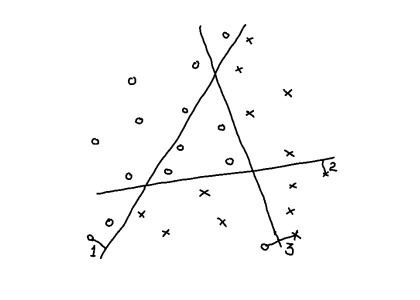
\includegraphics{MLbook/chapters/logical/images/logical.png} \caption{Построение решающего списка из трёх полуплоскостей.} \end{figure}

Непосредственное применение жадного алгоритма построения решающего списка к семейству предикатов семейства полуплоскостей позволяет построить покрытие обучающей выборки полуплоскостями. В этом случае решающий список описывает кусочно-линейную разделяющую поверхность между классами.

Известно большое количество эвристик для последовательного построения разделяющих полуплоскостей.

\textbf{Пример} Алгоритм Белледго строит полуплоскости, отделяющие как можно больше объектов одного класса, что равносильно максимизации информативности предиката, относящихся к параметрическому семейству полуплоскостей. Для этого применяются методы линейного программирования. В отличие от жадного алгоритма, после построения каждой полуплоскости делается попытка найти лучшие положения предыдущих полуплоскостей.

\textbf{Пример} В алгоритме Маршанда и др. перебираются всевозможные гиперплоскости, разделяющие какие-нибудь три точки (data dependent half-spaces), и из них выбирается полуплоскость с максимальной информативностью.

\subsection*{Достоинства решающих списков.}

\begin{itemize} \item Интерпретируемость и простота классификации. Обученное по выборке правило классификации можно записать в виде инструкции и выполнять «вручную». \item Гибкость: в зависимости от выбора множества $\Phi$ можно строить весьма разнообразные алгоритмические конструкции. \item Возможность обработки разнородных данных и данных с пропусками. \end{itemize}

\subsection*{Недостатки решающих списков.}

\begin{itemize} \item Если множество правил $\Phi$ выбрано неудачно, список может не построиться. При этом возможен высокий процент отказов от классификации. \item Возможна утрата интерпретируемости, если список длинный и правила различных классов следуют вперемежку. В этом случае правила не могут быть интерпретированы по-отдельности, без учёта предшествующих правил, и логика их взаимодействия становится довольно запутанной. \item Каждый объект классифицируется только одним правилом, что не позволяет правилам компенсировать неточности друг друга. Данный недостаток устраняется путём голосования правил, но это уже совсем другой алгоритм. \end{itemize}

\subsection*{Задачи}

\textbf{Задача 1.} Рассмотрим задачу построения решающего списка с использованием покрывающих шаров. Пусть у нас есть два класса $A$ и $B$ и множество объектов с координатами на плоскости:
A={(0,0),(1,0),(2,0)},B={(3,3),(4,3)}.
A={(0,0),(1,0),(2,0)},B={(3,3),(4,3)}.

Необходимо построить последовательность покрывающих шаров, начиная с класса $A$, так чтобы каждый последующий шар покрывал все объекты данного класса, но не пересекался с уже выделенными объектами другого класса. Найдите:

    Минимальный радиус шара, покрывающего все объекты класса $A$.

    Если этот шар пересекает хотя бы один объект класса $B$, постройте следующий шар для класса $B$ с наименьшим радиусом, покрывающим все оставшиеся объекты класса $B$.

\textbf{Решение 1.}
Минимальный шар, покрывающий точки $(0,0), (1,0), (2,0)$, будет иметь центр в точке $(1,0)$ и радиус $R_A = 1$. Он покрывает точки $(0,0)$ и $(2,0)$ за счёт расположения на прямой оси $x$. Поскольку объекты класса $B$ лежат далеко (в районе $(3,3)$ и $(4,3)$), они не входят в этот шар. Значит, нет пересечения с классом $B$ и можно зафиксировать первый шар радиусом $R_A = 1$. Далее для класса $B$ минимальный шар, покрывающий точки $(3,3)$ и $(4,3)$, будет иметь центр в точке $(3.5, 3)$ и радиус $R_B = 0.5$. В итоге получаем решающий список из двух шаров: первый для класса $A$ радиуса 1, второй для класса $B$ радиуса 0.5.

\medskip

\textbf{Задача 2.} Рассмотрим задачу построения решающего списка с использованием полуплоскостей. Пусть у нас есть выборка точек на плоскости:
A={(1,1),(2,1),(1,2)},B={(3,1),(3,2)}.
A={(1,1),(2,1),(1,2)},B={(3,1),(3,2)}.

Требуется найти полуплоскость, максимально отделяющую класс $A$ от $B$. То есть найдите такую линейную неравенство вида $w_1 x + w_2 y + b \geq 0$, что в одной полуплоскости окажется как можно больше точек класса $A$ и как можно меньше точек класса $B$.

\textbf{Решение 2.}
Опишем подход. Пусть мы хотим максимизировать число объектов класса $A$ в положительной полуплоскости и минимизировать число объектов класса $B$ в ней. Для решения подобной задачи можно сформулировать задачу линейного программирования: ввести индикаторные переменные, отвечающие за правильное отделение точек, и попытаться максимизировать суммарный «вес» классифицированных точек класса $A$ при ограничениях, не допускающих попадания многих точек класса $B$ в ту же полуплоскость. Геометрически для данного набора можно проверить несколько направлений: например, если взять прямую, проходящую между точками $(2,1)$ и $(3,1)$, под наклоном с положительным коэффициентом наклона, то удаётся поместить все точки $A$ в полуплоскость слева, а точки $B$ справа. Например, неравенство вида $x + y - 3 \geq 0$ поместит $(1,1)$ и $(1,2)$ в отрицательную полуплоскость (так как $1+1-3=-1<0$ и $1+2-3=0$ на границе), а $(2,1)$ в отрицательную ($2+1-3=0$ на границе). Выбирая чуть иное смещение, например $x + y - 2.5 \geq 0$, можно добиться того, чтобы все $A$ оказались по одну сторону, а $B$ — по другую. Таким образом, последовательно подбирая коэффициенты, добиваемся «лучшего» разделения классов.

\medskip

\textbf{Задача 3.} Рассмотрим решающий список из $N$ правил, где каждая строка — это предикат $\varphi_t(x)$ и соответствующий класс $c_t$. Предположим, что каждая проверка предиката занимает время $O(1)$, но интерпретация списка человеком усложняется пропорционально $N$. Пусть $N = 10$ — список довольно понятен, $N = 100$ — список уже трудно интерпретировать, а при $N = 1000$ практически невозможно понять логику классификации. Предположим, что каждая новая добавляемая строка увеличивает точность на 1%, но при этом на 10 единиц усложняет интерпретацию (условная метрическая оценка сложности).

    Определите, насколько уменьшится интерпретируемость при увеличении числа правил с $N = 10$ до $N = 1000$.

    При каком $N$ целесообразно остановиться с точки зрения баланса между точностью (+1% за правило) и интерпретируемостью (каждое правило добавляет 10 условных единиц сложности)?

\textbf{Решение 3.}
Если при $N=10$ сложность условно равна $10 \cdot 10 = 100$ единиц, то при $N=1000$ сложность будет $1000 \cdot 10 = 10000$ единиц. Интерпретируемость, обратно пропорциональная сложности, значительно упадёт, примерно в 100 раз, если считать, что интерпретируемость обратно пропорциональна числу правил.

    Если каждое правило добавляет 1\% к точности, то при увеличении с $10$ до $1000$ правил мы повысим точность на $990\%$, что не имеет смысла (точность не может превышать 100\%). Но если представить, что начальная точность была, скажем, 60\%, то до 100\% нам нужно всего 40 правил. Значит, достижение 100\% точности произойдёт уже при $N=50$. Проверим сложность: при $N=50$ сложность будет $50 \cdot 10 = 500$ единиц, что в 5 раз больше начального варианта с $N=10$. Это может быть приемлемым компромиссом. Таким образом, если нам не нужно «абсолютное» повышение точности, есть смысл остановиться при числе правил $N$, при котором точность уже удовлетворительна (например, близка к 100\%), а сложность ещё не стала слишком высокой.






\section{Взвешенное голосование правил}

Допустим, имеется консилиум экспертов, каждый член которого может допустить ошибку. Процедура голосования — это способ повышения качества принимаемых решений, при котором ошибки отдельных экспертов компенсируют друг друга.

Ранее принцип голосования применялся для построения композиций из произвольных алгоритмов классификации. Теперь рассмотрим композиции, состоящие из логических закономерностей.

\subsection{Принцип голосования}

Пусть для каждого класса $c \in Y$ построено множество логических закономерностей (правил), специализирующихся на различении объектов данного класса:

\[
R_c = \{ \varphi_{tc} : X \to \{0, 1\} \mid t = 1, \dots, T_c \}
\]

Считается, что если $\varphi_{tc}(x) = 1$, то правило $\varphi_{tc}$ относит объект $x \in X$ к классу $c$. Если же $\varphi_{tc}(x) = 0$, то правило воздерживается от классификации объекта $x$.

Алгоритм простого голосования (simple voting) подсчитывает долю правил в наборах $R_c$, относящих объект $x$ к каждому из классов:

\[
\Gamma_c(x) = \frac{1}{T_c} \sum_{t=1}^{T_c} \varphi_{tc}(x), \quad c \in Y,
\]

и относит объект $x$ к тому классу, за который подана наибольшая доля голосов:

\[
a(x) = \arg \max_{c \in Y} \Gamma_c(x).
\]

Если максимум достигается одновременно на нескольких классах, выбирается тот, для которого цена ошибки меньше.

Нормирующий множитель $\frac{1}{T_c}$ вводится для того, чтобы наборы с большим числом правил не перетягивали объекты в свой класс.

\subsection{Алгоритм взвешенного голосования}
Алгоритм взвешенного голосования (weighted voting, WV) действует более тонко, учитывая, что правила могут иметь различную ценность. Каждому правилу $\varphi_{tc}$ приписывается вес $\alpha_{tc} \geq 0$, и при голосовании берется взвешенная сумма голосов:

\[
\Gamma_c(x) = \sum_{t=1}^{T_c} \alpha_{tc} \varphi_{tc}(x), \quad \alpha_{tc} > 0.
\]

Веса нормируются на единицу:

\[
\sum_{t=1}^{T_c} \alpha_{tc} = 1, \quad \forall c \in Y.
\]

Поэтому функцию $\Gamma_c(x)$ называют также выпуклой комбинацией правил $\varphi_1, \dots, \varphi_{T_c}$. Очевидно, простое голосование является частным случаем взвешенного, когда веса одинаковы и равны $\frac{1}{T_c}$.

На первый взгляд, вес правила должен определяться его информативностью. Однако, важно также учитывать, насколько данное правило уникально. Если имеется 10 хороших, но одинаковых (или почти одинаковых) правил, их суммарный вес должен быть сравним с весом столь же хорошего правила, не похожего на все остальные. Таким образом, веса должны учитывать не только ценность правил, но и их различность.

Простой общий подход к настройке весов заключается в том, чтобы сначала найти набор правил $\{ \varphi_{tc}(x) \}$, затем принять их за новые (бинарные) признаки и построить в этом новом признаковом пространстве линейную разделяющую поверхность (кусочно-линейную, если $|Y| > 2$). Для этого можно использовать логистическую регрессию, однослойный персептрон или метод опорных векторов. Существуют и другие подходы. Например, в разделе 1.5.4 будет рассмотрен метод бустинга, в котором правила настраиваются последовательно, и для каждого правила сразу вычисляется его вес.

\subsection{Проблема диверсификации правил}
Голосующие правила должны быть существенно различны, иначе они будут бесполезны для классификации. Продолжая аналогию с консилиумом, заметим, что нет никакого смысла держать в консилиуме эксперта A, если он регулярно подсматривает решения у эксперта B.

Приведем простое теоретико-вероятностное обоснование принципа диверсификации, или повышения различности (diversity) правил \cite{14}. Пусть $X$ — вероятностное пространство, множество ответов $Y$ конечно. Введем случайную величину $M(x)$, равную перевесу голосов в пользу правильного класса; её называют также отступом (margin) объекта $x$ от границы классов:

\[
M(x) = \Gamma_c(x) - \Gamma_{\overline{c}}(x), \quad \Gamma_{\overline{c}}(x) = \max_{y \in Y \setminus \{c\}} \Gamma_y(x), \quad c = y^*(x).
\]

Если отступ положителен ($M(x) > 0$), то алгоритм голосования правильно классифицирует объект $x$. Предположим, что в среднем наш алгоритм классифицирует хотя бы немного лучше, чем наугад: $E[M] > 0$. Тогда можно оценить вероятность ошибки по неравенству Чебышева:

\[
P\{M < 0\} \leq P\{|E[M] - M| > E[M]\} \leq \frac{D_M}{(E[M])^2}.
\]

Отсюда вывод: для уменьшения вероятности ошибки необходимо максимизировать ожидание перевеса голосов $E[M]$ и минимизировать его дисперсию $D_M$. Для выполнения этих условий каждый объект должен выделяться примерно одинаковым числом правил. Обычно ни одно из правил не выделяет класс целиком, поэтому правила должны быть существенно различны, то есть выделять существенно различные подмножества объектов.

Неплохая эвристика, усиливающая различия между правилами и позволяющая равномернее выделять объекты обучения, используется в алгоритме CORAL \cite{12}. Сначала для фиксированного класса $c \in Y$ строится покрывающий набор правил точно так, как это делалось для решающих списков. Затем строится второй покрывающий набор, но при этом запрещается использовать признаки, часто входившие в закономерности первого набора. Поэтому второй набор неминуемо окажется отличным от первого. Затем запрещаются признаки, часто входившие в оба набора, и строится третий набор. И так далее, для каждого класса $c \in Y$.

\subsection{Отказы от классификации}
Возможны ситуации, когда ни одно из правил не выделяет классифицируемый объект $x$. Тогда алгоритм должен либо отказываться от классификации, либо относить объект к классу, имеющему наименьшую цену ошибки. Отказ алгоритма означает, что данный объект является нетипичным, не подпадающим ни под одну из ранее обнаруженных закономерностей. Вообще, обнаружение нетипичности (novelty detection) принято считать отдельным видом задач обучения по прецедентам, наряду с классификацией и кластеризацией. Способность алгоритмов отказываться от классификации нетипичных объектов во многих приложениях является скорее преимуществом, чем недостатком. В то же время, число отказов не должно быть слишком большим.

Итак, при построении алгоритмов взвешенного голосования правил возникает четыре основных вопроса:
\begin{itemize}
    \item Как построить много правил по одной и той же выборке?
    \item Как избежать повторов и построения почти одинаковых правил?
    \item Как избежать появления непокрытых объектов и обеспечить равномерное покрытие всей выборки правилами?
    \item Как определять веса правил при взвешенном голосовании?
\end{itemize}

Рассмотрим, как эти проблемы решаются в известных алгоритмах в следующих параграфах.

\subsection{Задачи}

\textbf{Задача 1: Алгоритм простого голосования}

Допустим, для класса $c \in Y$ существуют 10 правил, которые используют данные для классификации. Каждое правило возвращает 1 или 0 для объекта $x$. Если для объекта $x$ правила 3 и 7 верно классифицируют объект как класс $c$, а остальные возвращают 0, как будет рассчитана доля голосов для класса $c$?

\textbf{Решение:}  
Для класса $c$ доля голосов рассчитывается как сумма всех правил, которые классифицируют объект как класс $c$, делённая на общее количество правил. Если 10 правил, то:
\[
\Gamma_c(x) = \frac{1}{10} \left( 1 + 0 + 0 + 0 + 0 + 0 + 1 + 0 + 0 + 0 \right) = \frac{2}{10} = 0.2
\]
Таким образом, для объекта $x$ доля голосов для класса $c$ составит 0.2.

\textbf{Задача 2: Проблема с весами в алгоритме взвешенного голосования}

В алгоритме взвешенного голосования веса для каждого правила нормируются на единицу. Если для класса $c$ у нас есть 3 правила с весами $\alpha_1 = 0.5$, $\alpha_2 = 0.3$, и $\alpha_3 = 0.2$, как будет выглядеть итоговая сумма голосов $\Gamma_c(x)$, если объект $x$ классифицируется всеми тремя правилами как класс $c$?

\textbf{Решение:}  
Итоговая сумма голосов для класса $c$ рассчитывается по формуле:
\[
\Gamma_c(x) = \sum_{t=1}^{T_c} \alpha_{tc} \varphi_{tc}(x)
\]
где $\varphi_{tc}(x) = 1$, если правило классифицирует объект как класс $c$, и 0 в противном случае. Если все 3 правила классифицируют объект как $c$, то:
\[
\Gamma_c(x) = 0.5 + 0.3 + 0.2 = 1.0
\]

\textbf{Задача 3: Проблема диверсификации правил}

Какова вероятность ошибки при использовании алгоритма голосования, если все правила сильно похожи друг на друга (например, классифицируют одинаковые подмножества объектов)?

\textbf{Решение:}  
Если правила сильно похожи, то вероятность ошибки возрастает. В таких случаях, возможно, правило не будет существенно различать объекты, и алгоритм может ошибаться при классификации новых объектов. Чтобы уменьшить вероятность ошибки, правила должны быть разнообразными, то есть они должны выделять разные подмножества объектов. Для максимизации различий между правилами можно использовать метод, как в алгоритме CORAL, который строит покрывающие наборы правил, постепенно исключая часто встречающиеся признаки.

\textbf{Задача 4: Принцип диверсификации правил}

Пусть для объекта $x$ имеется 10 правил, из которых 8 классифицируют объект как класс $c$, а остальные 2 — как класс $d$. Какой отступ $M(x)$ будет при расчете вероятности правильной классификации?

\textbf{Решение:}  
Отступ для объекта $x$ определяется как разница между голосами для правильного класса и максимальным голосом для всех остальных классов:
\[
M(x) = \Gamma_c(x) - \Gamma_{\overline{c}}(x)
\]
Если из 10 правил 8 голосуют за класс $c$ (доля голосов $0.8$) и 2 — за класс $d$ (доля голосов $0.2$), то:
\[
M(x) = 0.8 - 0.2 = 0.6
\]
Если отступ положителен ($M(x) > 0$), то классификация будет правильной.

\textbf{Задача 5: Отказы от классификации}

Если для объекта $x$ не существует правила, которое его классифицирует, что должен делать алгоритм голосования? Как можно обработать такой случай?

\textbf{Решение:}  
В таком случае алгоритм может либо отказаться от классификации, либо отнести объект к классу с наименьшей ценой ошибки. Такой отказ от классификации часто называют обнаружением нетипичности (novelty detection), что является отдельной задачей в машинном обучении. Важно, чтобы количество отказов не было слишком большим, так как это может снизить эффективность алгоритма.

\section{Решающие списки}
\subsection{Опреление}
    Решающий список - это логический алгоритм классификации $a: X \xrightarrow{} Y$, задаваемый закономерностями $\varphi_1, \dots, \varphi_T$ классов $c_1, \dots, c_T \in Y$, вычисляемый следующим алоритмом

\hline
\begin{enumerate}
    \item \textbf{для всех} $t = 1, \dots, T_{max}$:
    \begin{itemize}
        \item \textbf{если} $\varphi_t(x) = 1$ 
        \begin{itemize}
            \item \textbf{вернуть $c_t$}
        \end{itemize}
    \end{itemize}
    
    \item \textbf{вернуть $c_0$}
\end{enumerate}
\hline
«Особый ответ» $c_0$ означает отказ алгоритма от классификации объекта $x$.
Обычно такие объекты приписывают классу, имеющему минимальную цену ошибки.
Например, в задаче выдачи кредитов отказ алгоритма приведёт к более осторожному решению «не выдавать». В задаче распознавания спама более осторожным будет
решение «не спам».

\textbf{Замечание} Соседние правила в списке $\varphi_{t-1}, \varphi_t$ можно переставлять местами,
если только они приписаны к одному классу, $c_{t-1} = c_t$. В общем случае перестановка
правил в списке изменяет алгоритм.

\subsection{Жадный алгоритм посторения}
Рассмотрим жадный алгоритм построения решающих списков.

Алгоритм, приведённый ниже, на каждой итерации строит ровно одно правило $\varphi_t$, выделяющее максимальное число объектов некоторого класса $c_t$ и минимальное число объектов
всех остальных классов. Для этого на каждой итерации производится поиск наиболее информативного правила $\varphi_t \in \Phi$, допускающего относительно мало ошибок. Семейство
правил $\Phi$ может быть каким угодно, лишь бы для него существовала эффективная
процедура поиска закономерностей. После построения правила $\varphi_t$ выделенные им объекты изымаются из выборки и алгоритм переходит к поиску следующего правила $\varphi_{t+1}$ по оставшимся объектам. В итоге выборка оказывается покрытой
множествами вида $\{x: \varphi_t(x) = 1\}$. Поэтому решающий список называют также покрывающим набором закономерностей или машиной покрывающих множеств.

\hline
\textbf{Вход:}
\begin{itemize}
    \item $X^l$ -- выборка;
    \item $T_{max}$ -- максимальное допустимое число правил в списке;
    \item $I_{min}$ -- минимальная допустимая информативность правил в списке;
    \item $E_{max}$ -- максимальная допустимая доля ошибок на обучающей выборке;
    \item $l_0$ -- максимальное допустимое число отказов.
\end{itemize}

\textbf{Выход:}
 $\{\varphi_1, \dots, \varphi_T\} \text{ — искомые решающие правила;}$

\hline
\begin{enumerate}
    \item $U := X^l;$
    \item \textbf{для всех} $i = 1, \dots, T_{max}$:
    \begin{itemize}
        \item \text{вычираем класс} $c := c_t$
        \item найти наиболее информативное правило при ограничении на долю ошибок:\
        $\varphi_t := \arg\min_{\varphi \in \Phi'} I_c(\varphi, U)$, где $\Phi' = \{ \varphi \in \Phi \ | \ E_c(\varphi, U) \leq E_{max} \}$ 

        \item \textbf{если} $I_c(\varphi_t, U) \leq I_{min}$ \textbf{то выход}
        \item Исключить из выборки объекты, выделенные правилом $\varphi_t$:
        $U := \{x \in U | \varphi_t(x) = 0\}$

        \item \textbf{если} $|U| \leq l_0$ \textbf{то выход}
    \end{itemize}
\end{enumerate}
\hline

\subsection{Анализ алгоритма}

\textbf{Критерии отбора правил.} Почему приходится использовать сразу два критерия
отбора правил $I_c$ и $E_c$? Правило с высокой информативностью $I_c$ вполне может допускать значительную долю ошибок $E_c$. Это нежелательно, так как в решающем списке каждое правило принимает окончательное решение. С другой стороны, правило с небольшой долей ошибок может выделять слишком мало объектов,
и по этой причине не являться закономерностью. Совместное использование обоих
критериев позволяет отобрать предикаты, удовлетворяющие условиям как статистической, так и логической закономерности.

\textbf{Критерии останова.} В данном алгоритме одновременно работают три критерия останова: 

(1) построение заданного числа правил $T_{max}$; 

(2) покрытие всей выборки, за исключением не более $l_0$ объектов; 

(3) невозможность найти правило с информативностью выше Imin по остатку выборки.

\textbf{Оптимизация сложности решающего списка.} Параметр $E_{max}$ позволяет найти
компромисс между точностью классификации обучающего материала и сложностью
списка. Уменьшение $E_{max}$ приводит к снижению числа ошибок на обучении. С другой
стороны, оно ужесточает отбор правил, способствует уменьшению числа объектов,
выделяемых отдельными правилами, и увеличению длины списка $T$. Правила, выделяющие слишком мало объектов, статистически не надёжны и могут допускать много
ошибок на независимых контрольных данных. Иными словами, увеличение длины
списка при одновременном «измельчении» правил может приводить к эффекту переобучения. Из общих соображений Emax должно быть приблизительно равно доле
ошибок, которую мы ожидаем получить как на обучающей выборке, так и вне её.
На практике параметр Emax подбирается экспериментально.

\textbf{Стратегия выбора класса.} Мы ничего не сказали о том, как выбирается класс $c_t$. Рассмотрим два варианта.
Первый вариант — сначала строятся все правила для первого класса, затем для второго, и так далее. Классы берутся в порядке убывания важности или цены ошибки. Преимущество данного варианта в том, что правила оказываются независимыми — в пределах своего класса их можно переставлять местами. Это улучшает
интерпретируемость правил.
Второй вариант — совместить 2 шага и выбирать пару $(\varphi_t
, c_t) \in \Phi \times Y$ , для
которой информативность $I_{c_t}(\varphi_t, U)$ максимальна. Тогда правила различных классов
могут следовать вперемежку. Доказано, что списки такого типа реализуют более широкое множество функций. При этом улучшается разделяющая способность
списка, но ухудшается его интерпретируемость.
На практике первый вариант часто оказывается более удобным. В некоторых случаях правила строятся только для $(M − 1)$ классов, а в последний, наименее
важный, класс $c_0$ объекты заносятся «по остаточному принципу».
Обработка пропусков в данных. Решающие списки позволяют легко обойти проблему пропущенных данных. Если для вычисления предиката 
$\varphi_t(x)$ не хватает данных, то считается, что $\varphi_t(x) = 0$, и обработку объекта $x$ берут на себя следующие
правила в списке. Это относится и к стадии обучения, и к стадии классификации.

\subsection{Разновидности решающих списков}
Логику решающего списка или, что то же самое, комитета старшинства, имеют
многие алгоритмы, предлагавшиеся в разное время разными авторами под разными названиями. Многочисленные варианты отличаются выбором семейства предикатов $\Phi$, критерием информативности и методом поиска информативных предикатов.

\textbf{Пример} Наиболее распространены решающие списки конъюнкций. Они почти
идеально соответствуют человеческой логике принятия решений, основанной на последовательной проверке достаточно простых правил. Поэтому решающие списки
часто используются для представления знаний, извлекаемых непосредственно из эмпирических данных. Для построения отдельных правил можно использовать жадный алгоритм, применяя для поиска $\varphi$ любой из методов поиска информативных конъюнкций,
например.

\textbf{Пример} В алгоритме Маршанда перебираются всевозможные гиперплоскости, разделяющие какие-нибудь три точки (data dependent half-spaces), и из них выбирается полуплоскость с максимальной информативностью.

\subsection{Достоинства и недостатки}

\textbf{Достоинства решающих списков.}
\begin{enumerate}
    \item Интерпретируемость и простота классификации. Обученное по выборке правило классификации можно записать в виде инструкции и выполнять «вручную».
    \item Гибкость: в зависимости от выбора множества $\Phi$ можно строить весьма разнообразные алгоритмические конструкции.
    \item Возможность обработки разнотипных данных и данных с пропусками.
\end{enumerate}
\\
\textbf{Недостатки решающих списков.}
\begin{enumerate}
    \item Если множество правил $\Phi$ выбрано неудачно, список может не построиться. При этом возможен высокий процент отказов от классификации.
    \item Возможна утрата интерпретируемости, если список длинный и правила различных классов следуют вперемежку. В этом случае правила не могут быть
    интерпретированы по-отдельности, без учёта предшествующих правил, и логика их взаимодействия становится довольно запутанной.
    \item Каждый объект классифицируется только одним правилом, что не позволяет
    правилам компенсировать неточности друг друга. Данный недостаток устраняется путём голосования правил, но это уже совсем другой алгоритм.
\end{enumerate}

\subsection{Задачи}

\textbf{Задача 1}
Постройте решающий список для логической функции $x \vee y \vee \overline{z}.$

\textbf{Решение}

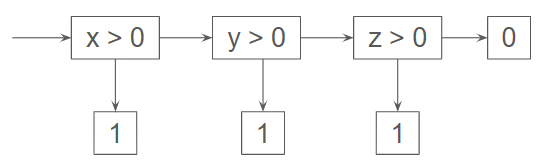
\includegraphics[scale = 0.5]{images/decide_list_task1_sol.png}

\textbf{Задача 2}
Адаптируйте решающий список для задач регрессии.

\textbf{Решение}
Давайте разобъём множество значений искомой зависимости $y: X \rightarrow{} Y$ на $T + 1$ множеств вида:
$[y < d_1], [d_1 \leq y < d_2], ..., [d_{T-1} \leq y < d_T], [d_T \leq y].$ 
Сопоставим эти множества с классами $c_1, \dots, c_T$.

Теперь запустим алгоритм построения решающего списка для полученных классов, 
но помимо нахождения правил $\varphi$, будем так же находить среднее значение $y$ на объектах, которые удовлетворяют этому правилу.
И будем выдавать по объекту $x$ среднее значение для объектов этого класса.

\section {Решающие таблицы}
\subsection{Опреление}

Решающая таблица - это частный стлучай решающего дерева глубины $H$, для всех узлов уровня $h$ условия ветвления $f_h(x)$ одинаковы. На уровне $h$ ровно $2^{h-1}$ вернин. $X$ делится на $2^H$ "ячеек".

\textbf{Пример.} Задача XOR, $H = 2$.

    \includegraphics[scale = 0.5]{images/decide_table_exapmle.png}

\subsection{Жадный алгоритм посторения}
Рассмотрим жадный алгоритм построения решающей таблицы

\hline
\textbf{Вход:}
\begin{itemize}
    \item $X^l$ — выборка;
    \item $F$ - множество признаков ;
    \item $H$ - глубина дерева.
\end{itemize}

\textbf{Выход:}
\begin{itemize}
    \item $\{f_1, \dots, f_H\};$ 
    \item таблица $T: \{0, 1\}^H \xrightarrow{} Y$
\end{itemize}

\hline
\begin{enumerate}
    \item $U := X^l;$
    \item \textbf{для всех} $h = 1, \dots, H$:
    \begin{itemize}
        \item предикат с максимальным выигрышем определённости:
        $f_h := \arg\min_{f \in F} Gain(f_1, \dots, f_{h-1}, f)$
    \end{itemize}
    \item классификация по мажоритарному правилу 
    $ T(\beta) := Major(U_{H\beta}) $
\end{enumerate}
\hline
Выигрыш от ветвления на уровне $h$ по всей выборке $X^L$:
$$Gain(f_1, \dots, f_h) = \Phi(X^l) - \sum_{\beta\in \{0, 1\}^h} \frac{U_{h\beta}}{l}\Phi(U_{h\beta})$$

$U_{h\beta} = \{ x_i \in X^l \ | \ f_s(x_i)=\beta_s,\ s=1\dots h \}, \beta=(\beta_1, \dots, \beta_h) \in \{0, 1\}^h$

$p_y =\frac{1}{|U|} \sum_{x_i \ in U}[y_i = y]$ -- частичная оценка $P(y|U)$.

$\Phi(U)$ -- мера неопределённости распределения $p_y$:
\begin{enumerate}
    \item минимальная  равна нулю, когда $p_y \in \{0,1\}$
    \item ксимальна, когда $p_y = \frac{1}{|Y|}$ -- номерное распределение
    \item симметрична, то есть не зависи от перенумерации классов
\end{enumerate}

\subsection{Задачи}

\textbf{Задача}
Постройте решающую таблицу для логической функции $x \vee (y \wedge \overline{z}).$ Изобразите её ввиде дерева.

\textbf{Решение}
\begin{figure}
    \centering
    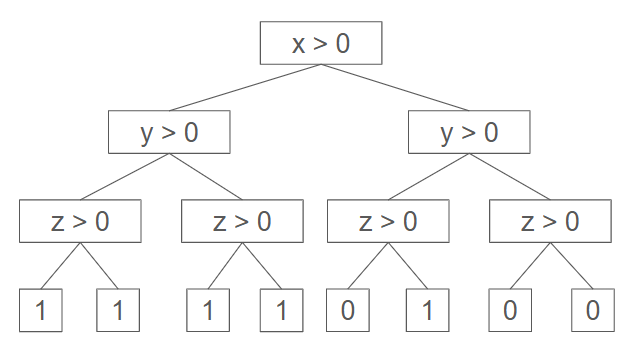
\includegraphics[width=0.5\linewidth]{decide_table_task_sol.png}
\end{figure}

\section{Алгоритм КОРА}

Алгоритм комбинаторного распознавания КОРА, предложенный М.М.~Бонгардом в 1961 году и реализованный М.Н.~Вайнцвайгом, предназначен для построения набора конъюнктивных закономерностей. Этот алгоритм неоднократно демонстрировал высокую эффективность при решении различных прикладных задач, связанных с распознаванием образов и классификацией.

\subsection{Основные эвристические предположения}

Для эффективной работы алгоритма КОРА сделаны следующие эвристические предположения:

\begin{itemize}
    \item \textbf{Адекватность множества предикатов:} Множество элементарных предикатов \(B\) выбрано таким образом, что среди конъюнкций ранга 2 или 3 уже содержится достаточное количество информативных закономерностей.
    \item \textbf{Ограничение ранга конъюнкций:} Поскольку ранг конъюнкций ограничен числом 3, для поиска закономерностей возможно применение полного перебора, что упрощает процесс поиска.
    \item \textbf{Непротиворечивость закономерностей:} Наибольший интерес представляют те закономерности, которые являются непротиворечивыми, то есть не содержат противоречий в данных.
\end{itemize}

\subsection{Пример дерева перебора}

На рисунке \ref{fig:kora_tree} показано дерево полного перебора конъюнкций в алгоритме КОРА при \(|B| = 4\). Для краткости конъюнкции обозначены номерами составляющих их предикатов.

\begin{figure}[h]
    \centering
    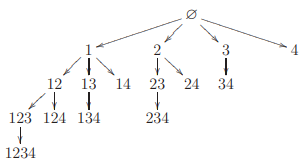
\includegraphics[width=0.6\textwidth]{images/kora_tree.png}
    \caption{Дерево полного перебора конъюнкций в алгоритме КОРА при \(|B| = 4\). Для краткости конъюнкции обозначены номерами составляющих их предикатов.}
    \label{fig:kora_tree}
\end{figure}

\subsection{Описание алгоритма}

Алгоритм КОРА строит конъюнкции, состоящие не более чем из \(K\) термов, выбранных из множества предикатов \(B\). Основой алгоритма является рекурсивная процедура \textit{Нарастить}(\(\varphi\)), которая добавляет термы в конъюнкцию \(\varphi(x)\) всевозможными способами. При этом в список закономерностей \(R_c\) заносятся только наиболее информативные конъюнкции.

\subsubsection{Параметры алгоритма}

Алгоритм использует следующие параметры:

\begin{itemize}
    \item \(D_{\text{min}}\) — минимальная доля позитивных объектов для конъюнкций.
    \item \(E_{\text{max}}\) — максимальная допустимая доля ошибок.
    \item \(T_{\text{min}}, T_{\text{max}}\) — ограничения на количество конъюнкций в списке.
\end{itemize}

\subsubsection{Построение списка информативных конъюнкций методом поиска в глубину (алгоритм КОРА)}

\textbf{Входные данные:}
\begin{itemize}
    \item \(X_\ell\) — обучающая выборка;
    \item \(B\) — семейство элементарных предикатов;
    \item \(K\) — максимальный ранг конъюнкций;
    \item \(E_{\text{max}}\) — максимальная доля ошибок \(E_c(\varphi)\) для конъюнкций \(\varphi \in R_c\);
    \item \(D_{\text{min}}\) — минимальная доля позитивных объектов \(D_c(\varphi)\) для конъюнкций \(\varphi \in R_c\);
    \item \(T_{\text{min}}, T_{\text{max}}\) — ограничения на количество конъюнкций \(T_c\).
\end{itemize}

\textbf{Выходные данные:} 
Списки конъюнкций \(R_c = \{ \varphi_{tc}(x) : t = 1, \dots, T_c \}, \) для всех \(c \in Y\).

\begin{enumerate}
    \item Инициализировать списки: \(R_c = \emptyset\) для всех \(c \in Y\).
    \item Повторять:
    \begin{itemize}
        \item Выполнить \textit{Нарастить}(\(\emptyset\));
        \item Определить \(T := \min_{c \in Y} |R_c|\);
        \item Если \(T < T_{\text{min}}\), то уменьшить \(D_{\text{min}}\) и/или увеличить \(E_{\text{max}}\);
        \item Если \(T > T_{\text{max}}\) или время поиска становится слишком большим, то увеличить \(D_{\text{min}}\) и/или уменьшить \(E_{\text{max}}\);
    \end{itemize}
    \item Пока \(T \notin [T_{\text{min}}, T_{\text{max}})\).
\end{enumerate}

\subsubsection{Процедура \textit{Нарастить}(\(\varphi\))}

\begin{enumerate}
    \item Если \(\varphi = \emptyset\), установить \(j_s := 0\).
    \item Для всех \(j \in \{ j_s + 1, \dots, |B| \}\):
    \begin{itemize}
        \item Добавить терм \(\beta_j\) к исходной конъюнкции:
        \[
        \varphi' := \varphi \wedge \beta_j
        \]
        \item Если \(|\varphi'| \leq K\) и существует \(c \in Y\), такое что:
        \[
        D_c(\varphi') > D_{\text{min}} \quad \text{и} \quad E_c(\varphi') \leq E_{\text{max}},
        \]
        то добавить \(\varphi'\) в список \(R_c\).
        \item Иначе, если \(|\varphi'| < K\) и существует \(c \in Y\), такое что \(D_c(\varphi') > D_{\text{min}}\), то рекурсивно вызвать \textit{Нарастить}(\(\varphi'\)).
    \end{itemize}
\end{enumerate}

\subsubsection{Включение конъюнкции \(\varphi\) в список \(R_c\), содержащий не менее \(T\) самых информативных конъюнкций}

Этот алгоритм предназначен для поддержания в списке \(R_c\) не менее \(T\) самых информативных конъюнкций. Эта процедура обеспечивает управление количеством конъюнкций в списке и поддержание их порядка по информативности.

\begin{enumerate}
    \item \textbf{Процедура} \textit{Добавить\_в\_список}( \(R_c\), \(\varphi\), \(T\) ):
    \item Вставить конъюнкцию \(\varphi\) в список \(R_c\) в порядке убывания информативности \(I_c(\varphi)\).
    \item Найти наименьшую информативность в списке:
    \[
    J := \min_{\psi \in R_c} I_c(\psi)
    \]
    \item Определить количество конъюнкций с наименьшей информативностью:
    \[
    \Delta := \#\{ \psi \in R_c : I_c(\psi) = J \}
    \]
    \item Если \(|R_c| - \Delta > T\), то удалить из списка \(R_c\) все конъюнкции с информативностью \(J\).
\end{enumerate}

\subsection{Достоинства алгоритма КОРА}

\begin{itemize}
    \item \textbf{Интерпретируемость:} Короткие конъюнкции легко интерпретируются в терминах предметной области.
    \item \textbf{Эффективность:} При малых значениях \(K\) (например, \(K \leq 3\)) алгоритм работает очень эффективно.
    \item \textbf{Полнота:} Если существуют короткие информативные конъюнкции, алгоритм обязательно их найдет.
\end{itemize}

\subsection{Недостатки алгоритма КОРА}

\begin{itemize}
    \item \textbf{Зависимость от предикатов:} При неудачном выборе множества предикатов \(B\) короткие информативные конъюнкции могут отсутствовать.
    \item \textbf{Экспоненциальная сложность:} Увеличение числа \(K\) приводит к экспоненциальному росту вычислительной сложности.
    \item \textbf{Отсутствие диверсификации:} Алгоритм не стремится диверсифицировать конъюнкции и обеспечивать равномерное покрытие объектов.
\end{itemize}

\section{Алгоритм ТЭМП}

Полный перебор всех конъюнкций ранга не более $K$ требует экспоненциального по $K$ числа операций. В реальных задачах объём вычислений становится огромным уже при $K > 3$, и от идеи полного перебора приходится отказаться.

Существует две стандартные стратегии перебора конъюнкций: поиск в глубину (depth-first search) и поиск в ширину (breadth-first search). Первая применяется в алгоритме КОРА, вторая — в алгоритме ТЭМП, предложенным Г. С. Лбовым в 1976 году. Поиск в ширину работает немного быстрее, и в него легче встраивать различные эвристики, сокращающие перебор.

В исходном варианте алгоритм ТЭМП выполнял полный перебор всех конъюнкций ранга не более $K$. Ниже описан слегка модифицированный вариант, позволяющий ограничить перебор и увеличить максимальный ранг конъюнкций $K$.

Алгоритм 1.9 начинает процесс поиска закономерностей с построения конъюнкций ранга 1. Для этого отбираются не более $T_1$ самых информативных предикатов из базового множества $\mathcal{B}$. Затем к каждому из отобранных предикатов добавляется по одному терму из $\mathcal{B}$ всеми возможными способами. Получается не более $T_1|\mathcal{B}|$ конъюнкций ранга 2, из которых снова отбираются $T_1$ самых информативных. И так далее. На каждом шаге процесса делается попытка добавить один терм к каждой из имеющихся конъюнкций. Наращивание конъюнкций прекращается либо при достижении максимального ранга $K$, либо когда ни одну из конъюнкций не удаётся улучшить путём добавления терма.

Лучшие конъюнкции, собранные со всех шагов, заносятся в списки $R_c$. Таким образом, списки $R_c$ могут содержать конъюнкции различного ранга.

Параметр $T_1$ позволяет найти компромисс между качеством и скоростью работы алгоритма. При $T_1 = 1$ алгоритм ТЭМП работает исключительно быстро и строит единственную конъюнкцию, добавляя термы по очереди. Фактически, он совпадает с жадным Алгоритмом 1.2. При увеличении $T_1$ пространство поиска расширяется, алгоритм начинает работать медленнее, но находит больше информативных конъюнкций. На практике выбирают максимальное значение параметра $T_1$, при котором поиск занимает приемлемое время. Однако стратегия поиска всё равно остаётся жадной — термы оптимизируются по-отдельности, и при подборе каждого терма учитываются только предыдущие, но не последующие термы.

Для улучшения конъюнкций к ним применяют эвристические методы «финальной шлифовки» — стабилизацию и редукцию.

В результате стабилизации конъюнкции становятся локально неулучшаемыми. Алгоритм в целом становится более устойчивым — при незначительных изменениях в составе обучающей выборки он чаще находит одни и те же закономерности, а значит, улучшается его способность обобщать эмпирические факты.

В результате стабилизации некоторые конъюнкции могут совпасть, и в списке появятся дубликаты. Их удаление предусмотрено на шаге 13. Если список $R_c$ поддерживается отсортированным по информативности, то удаление дубликатов является недорогой операцией, так как достаточно проверять на совпадение только соседние конъюнкции с одинаковой информативностью.

Если задать $T_1 = \infty$, то алгоритм выполнит полный перебор, как в исходном варианте ТЭМП. «Финальная шлифовка» в этом случае не нужна.

\subsection{Алгоритм 1.9. Построение списка информативных конъюнкций методом поиска в ширину (алгоритм ТЭМП)}


\subsection{Алгоритм 1.9: Построение списка информативных конъюнкций методом поиска в ширину}

\textbf{Вход:}
\begin{itemize}
    \item $X_\ell$ --- обучающая выборка;
    \item $\mathcal{B}$ --- семейство элементарных предикатов;
    \item $c \in Y$ --- класс, для которого строится список конъюнкций;
    \item $K$ --- максимальный ранг конъюнкций;
    \item $T_1$ --- число лучших конъюнкций, отбираемых на каждом шаге;
    \item $T_0$ --- число лучших конъюнкций, отбираемых на последнем шаге, $T_0 \leq T_1$;
    \item $I_{\min}$ --- порог информативности;
    \item $E_{\max}$ --- порог допустимой доли ошибок;
    \item $X_k$ --- контрольная выборка для проведения редукции.
\end{itemize}

\textbf{Выход:} Список конъюнкций $R_c = \{\varphi_t^c(x) : t = 1, \dots, T_c\}$.

\begin{enumerate}
    \item $R_c \gets \emptyset$;
    \item Для всех $\beta \in \mathcal{B}$: \texttt{Добавить\_в\_список($R_c$, $\beta$, $T_1$)};
    \item Для всех $k = 2, \dots, K$:
    \begin{enumerate}
        \item Для всех конъюнкций $\varphi \in R_c$ ранга $(k-1)$:
        \begin{enumerate}
            \item Для всех предикатов $\beta \in \mathcal{B}$, которых ещё нет в конъюнкции $\varphi$:
            \begin{enumerate}
                \item Добавить терм $\beta$ к конъюнкции $\varphi$: $\varphi' = \varphi \land \beta$;
                \item Если $I_c(\varphi') > I_{\min}$, $E_c(\varphi') \leq E_{\max}$ и конъюнкции $\varphi'$ нет в $R_c$, то \texttt{Добавить\_в\_список($R_c$, $\varphi'$, $T_1$)}.
            \end{enumerate}
        \end{enumerate}
    \end{enumerate}
    \item Для всех конъюнкций $\varphi \in R_c$:
    \begin{enumerate}
        \item Стабилизация($\varphi$);
        \item Редукция($\varphi$, $X^k$);
    \end{enumerate}
    \item Удалить из списка $R_c$ дублирующие конъюнкции;
    \item Оставить в списке $R_c$ не более $T_0$ лучших конъюнкций.
\end{enumerate}


\subsection{Достоинства алгоритма ТЭМП}

\begin{itemize}
    \item ТЭМП существенно более эффективен, чем КОРА, особенно при поиске конъюнкций ранга больше 3. Он решает поставленную задачу за $O(KT_1|B|\\ell)$ операций, тогда как КОРА имеет трудоёмкость $O(|B|K\\ell)$.
    \item Параметр $T_1$ позволяет управлять жадностью алгоритма и находить компромисс между качеством конъюнкций и скоростью работы алгоритма.
    \item Благодаря простоте и эффективности алгоритм ТЭМП можно использовать в составе других алгоритмов как генератор конъюнкций, достаточно близких к оптимальным.
\end{itemize}

\subsection{Недостатки алгоритма ТЭМП}

\begin{itemize}
    \item Нет гарантии, что будут найдены самые лучшие конъюнкции, особенно при малых значениях параметра $T_1$.
    \item Алгоритм не стремится увеличивать различность конъюнкций, добиваясь равномерного покрытия объектов выборки. Стабилизация и редукция лишь отчасти компенсируют этот недостаток.
    \item Нет настройки коэффициентов $\\alpha_{tc}$; предполагается простое голосование.

\end{itemize}

\subsection{Задачи}

\textbf{Задача 1}  
Рассмотрим множество элементарных предикатов \( B = \{ \beta_1, \beta_2, \beta_3 \} \) и обучающую выборку \( X_\ell \) с классами \( Y = \{A, B\} \). Предположим, что следующие конъюнкции удовлетворяют условиям \( D_{\text{min}} \) и \( E_{\text{max}} \):

\[
\varphi_1 = \beta_1 \wedge \beta_2, \quad \varphi_2 = \beta_2 \wedge \beta_3, \quad \varphi_3 = \beta_1 \wedge \beta_3
\]

Определите, какие из этих конъюнкций будут добавлены в списки \( R_A \) и \( R_B \) после выполнения процедуры \textit{Нарастить}(\(\emptyset\)).

\textbf{Решение}  
Процедура \textit{Нарастить} начинает с пустой конъюнкции и добавляет термы по одному. Проверяем каждую конъюнкцию на удовлетворение условий \( D_{\text{min}} \) и \( E_{\text{max}} \):

\begin{itemize}
    \item \(\varphi_1 = \beta_1 \wedge \beta_2\): Если для класса \(A\) \(D_A(\varphi_1) > D_{\text{min}}\) и \(E_A(\varphi_1) \leq E_{\text{max}}\), то \(\varphi_1\) добавляется в \( R_A \). Аналогично проверяется для класса \(B\).
    \item \(\varphi_2 = \beta_2 \wedge \beta_3\): Аналогично, добавляется в соответствующие списки классов.
    \item \(\varphi_3 = \beta_1 \wedge \beta_3\): Аналогично, добавляется в соответствующие списки классов.
\end{itemize}

Таким образом, все три конъюнкции будут добавлены в списки \( R_A \) и \( R_B \), если они удовлетворяют заданным условиям.

\textbf{Задача 2}  
Предположим, что при использовании алгоритма КОРА параметр \( K \) увеличен с 3 до 4. Объясните, как это повлияет на эффективность алгоритма и количество генерируемых конъюнкций.

\textbf{Решение}  
Увеличение параметра \( K \) с 3 до 4 расширяет максимальный ранг конъюнкций, позволяя создавать более сложные правила с дополнительным термом. Однако это приводит к экспоненциальному росту числа возможных конъюнкций, что значительно снижает эффективность алгоритма из-за увеличения вычислительной сложности. Кроме того, при большем \( K \) может возрастать вероятность переобучения, так как алгоритм будет генерировать больше конъюнкций, что может привести к снижению обобщающей способности модели.

\textbf{Задача 3}  
Рассмотрим ситуацию, когда множество предикатов \( B \) плохо выбрано, и среди конъюнкций ранга 2 или 3 отсутствуют информативные закономерности. Как это повлияет на работу алгоритма КОРА и какие меры можно предпринять для улучшения результатов?

\textbf{Решение}  
Если множество предикатов \( B \) плохо выбрано и среди конъюнкций ранга 2 или 3 отсутствуют информативные закономерности, алгоритм КОРА не сможет эффективно выявить необходимые закономерности, что приведет к низкой точности классификации. Для улучшения результатов можно предпринять следующие меры:

\begin{enumerate}
    \item \textbf{Пересмотр множества предикатов \( B \):} Добавить новые предикаты или изменить существующие, чтобы повысить их информативность.
    \item \textbf{Увеличение максимального ранга \( K \):} Хотя это снижает эффективность, иногда требуется более высокий ранг для захвата сложных закономерностей.
    \item \textbf{Использование методов отбора признаков:} Применить методы отбора признаков для выбора наиболее информативных предикатов, что может улучшить качество конъюнкций.
    \item \textbf{Комбинирование с другими алгоритмами:} Интегрировать КОРА с другими алгоритмами машинного обучения для улучшения общего качества модели.
\end{enumerate}

Эти меры помогут повысить информативность конъюнкций и, соответственно, эффективность алгоритма КОРА.

\textbf{Задача 1.}
\newline
Рассмотрите граф $G = (V, E)$, где $V = \{A, B, C, D, E\}$ и $E = \{(A, B), (A, C), (B, D), (C, D), (D, E)\}$. Как алгоритм ТЭМП выполняет поиск в ширину для этого графа? Предложите, как можно выполнить поиск в глубину.

\textit{Решение:}
\begin{enumerate}
    \item Алгоритм ТЭМП начинает с вершины $A$, добавляя её соседей $B$ и $C$ в очередь. Затем из очереди выбирается вершина $B$, её сосед $D$ добавляется в очередь, и так далее.
    \item Для поиска в глубину из вершины $A$ алгоритм выбирает один путь (например, $A \to B \to D \to E$), пока не дойдёт до конца, затем возвращается и ищет другие пути.
\end{enumerate}

\textbf{Задача 2.}
\newline
Пусть у нас есть множество предикатов $B = \beta_1, \beta_2, \beta_3$ и максимальный ранг $K = 2$. Какое количество конъюнкций будет проверено алгоритмом ТЭМП, если для каждого шага выбирается $T_1 = 2$? Если мы увеличим $T_1$ до 3, как это повлияет на количество проверяемых конъюнкций?

\textit{Решение:}
\begin{itemize}
    \item При $T_1 = 2$ для ранга 1 будет 2 конъюнкции, для ранга 2 --- $2 \times 3 = 6$ конъюнкций. Всего будет проверено $2 + 6 = 8$ конъюнкций.
    \item Если $T_1 = 3$, то для ранга 1 будет 3 конъюнкции, для ранга 2 --- $3 \times 3 = 9$ конъюнкций. Всего будет проверено $3 + 9 = 12$ конъюнкций.
\end{itemize}

\textbf{Задача 3.}
\newline
Представьте, что вы используете алгоритм ТЭМП для обучения модели с большим количеством предикатов. Какой будет влияние на время вычислений, если вы увеличите $T_1$ с 1 до 5? Объясните это с точки зрения расширения пространства поиска.

\textit{Решение:}
\begin{itemize}
    \item При $T_1 = 1$ алгоритм будет проверять только по одному терму для каждой конъюнкции на каждом шаге, что будет довольно быстрым, но может не давать лучшие результаты.
    \item При увеличении $T_1$ до 5 пространство поиска расширяется, так как на каждом шаге будет добавляться больше термов к конъюнкциям, что увеличивает количество проверяемых комбинаций и тем самым замедляет процесс.
    \item В результате увеличение $T_1$ может существенно замедлить алгоритм, но при этом улучшится качество найденных решений.
\end{itemize}


\section{Решающие деревья регрессии.}

Деревья регрессии - тип деревьев решений. Он используется в случае, когда целевой признак является непрерывным, например, действительным числом. Дерево имеет два типа вершин:
\begin{itemize}
    \item Внутренние вершины, переходы из которых осуществляются при помощи применения предикатов к признакам объекта.
    \item Листья, содержащие предсказания целевого признака. При этом значения для листьев вычисляются на этапе обучения как функция от значений целевого признака для всех объектов тренировочной выборки, попадающих в эту вершину. В отличие от классифицирующего дерева, здесь получается конкретное значение, а не класс и не вектор вероятностей принадлежности к классам.
\end{itemize}
Таким образом, регрессионные решающие деревья позволяют получать приближения целевой функции при помощи кусочно-постоянных функций.

\subsection{Построение регрессионных решающих деревьев}
Для построения регрессионных деревьев используется алгоритм CART (Classification And Regression Trees). Сначала нужно выбрать критерий разбиения, то есть меру неопределенности, которую мы будем минимизировать при поиске наилучшего способа разбить вершину.

\subsubsection{Метрики построения}
В случае регрессионных решающих деревьев используются метрики, подходящие для непрерывных значений целевого признака. Среди них наиболее популярны MSE и MAE:
\begin{itemize}
    \item  Средняя квадратичная ошибка (MSE): Измеряет среднюю квадратичную разницу между наблюдаемыми и предсказанными значениями на тренировочной выборке:
    \begin{align*}
        MSE = \frac{1}{n} \sum_{i=1}^{n} (y_i - \hat{y}_i)^2
    \end{align*} 
    \item Средняя абсолютная ошибка (MAE): Измеряет среднюю абсолютную разницу между наблюдаемыми и прогнозируемыми значениями на тренировочной выборке.
    \begin{align*}
        MAE = \frac{1}{n} \sum_{i=1}^{n} |y_i - \hat{y}_i|
    \end{align*}
\end{itemize}

Зачастую для избежания переобучения к минимизируемой функции также добавляется штраф, связанный с числом вершин в дереве.

\subsubsection{Процесс построения}
После выбора метрики осуществляется жадное рекурсивное построение дерева. На каждом шаге выбирается вершина, и задача заключается в выборе такого предиката, который бы разбивал множество приходящих в неё объектов обучающей выборки наилучшим с точки зрения минимизации метрики ошибки способом. Для этого перебираются все признаки, и для каждого признака подбирается оптимальное пороговое значение, после чего выбирается признак, дающий наилучший результат. В случае, если ни одно из разбиений не даёт подходящего результата, вершина остаётся листом. Также разбиение может прекратиться в случае, если установлено ограничение на количество вершин.

Для рекурсивного выполнения алгоритма процесс запускается из корневой вершины, после чего при каждом разбиении последующей вершины запускается также для её дочерних вершин.

\subsubsection{Усечение ветвей}

Решающие деревья склонны к переобучению из-за того, что с увеличением глубины каждую вершину достигает всё меньшее число объектов. Для решения этой проблемы используется усечение ветвей (pruning). Идея заключается в проверке работы дерева на данных, не использовавшихся при обучении, и отбрасывании поддеревьев с большой ошибкой. Чтобы применить этот метод, нужно изначально выделить часть обучающей выборки, которая будет использоваться только при прунинге.

Различают два подхода к усечению ветвей: обход дерева от корня к листьям и от листьев к корню.     

\begin{itemize}
    \item Top-down pruning — подход, при котором проверка и обрезка наименее информативных ветвей начинается с корневого узла. Данный метод обладает относительно низкой вычислительной сложностью, однако может приводить к недообучению за счёт удаления ветвей, которые могли потенциально содержать информативные узлы. В качестве примера можно привести Pessimistic Error Pruning (PEP). При таком подходе удаляются поддеревья с наибольшей ошибкой на отложенной выборке, порог устанавливается заранее.
    
    \item Bottom-up pruning — подход, при котором проверка и обрезка наименее информативных ветвей начинается с листьев. В данном случае получаются более точные деревья за счёт оценки каждого узла по отдельности. Но из-за полного обхода дерева увеличивается вычислительная сложность. Среди методов данного подхода можно выделить следующие:
    \begin{itemize}
        \item Reduced Error Pruning (REP), когда решающие узлы удаляются до тех пор, пока не падает точность, измеренная на отложенной выборке;

        \item Cost-complexity pruning (CCP), когда последовательно строится серия поддеревьев исходного дерева через удаление слабейших узлов. После этого наилучшее дерево можно выбрать при проверке на тестовой выборке.
    \end{itemize}
\end{itemize}

При усечении поддерева можно использовать один из следующих вариантов:
\begin{itemize}
    \item Оставить поддерево без изменений,
    \item Заменить поддерево одним из дочерних,
    \item Объединить дочерние поддеревья и заново рассчитать предсказание.
\end{itemize}
Выбор происходит с точки зрения минимизации меры неопределенности.

\subsection{Преимущества и недостатки регрессионных решающих деревьев}

В качестве преимуществ решающих деревьев регрессии стоит выделить:
\begin{itemize}
    \item Интерпретируемость. Последовательный анализ признаков с учетом результатов применения предыдущих предикатов схож с процессом мышления человека.
    \item Алгоритмическая сложность использования. Количество операций пропорционально глубине дерева, а сравнение -- быстрая операция, что позволяет неглубоким деревьям работать быстро.
    \item Определение наиболее важных признаков. В процессе построения разбиение начинается с признаков, дающих наибольшую информацию об объекте, и решающие деревья хорошо справляются с ситуацией, когда часть признаков информативнее других.
    \item Приближение нелинейных зависимостей. Кусочно-линейные функции позволяют сколь угодно хорошо приблизить большое количество функций и не требуют предварительного анализа характера зависимости.
\end{itemize}

Недостатки регрессионных решающих деревьев:
\begin{itemize}
    \item Сложность построения. В общем случае для поиска оптимального дерева необходимо перебирать все возможные варианты деревьев, что является np-полной задачей.
    \item Чувствительность к выбросам. Поскольку деревья решений разбивают выборку на подмножества исходя из минимизации значения метрики, они могут выделять выбросы с сильно отличающимися от остальных значениями, что значительно уменьшает штраф. В таком случае для объектов, находящиеся вблизи выброса, будут сделаны неверные предсказания. 
    \item Переобучение. Из-за того, что к глубоким вершинам относятся всё меньшие по мощности подмножества обучающей выборки, дерево может переобучиться под конкретные элементы. Для этого приходится проводить пост-обработку, устанавливать ограничение на число вершин, или включать дополнительные штрафы в минимизируемую функцию.
\end{itemize}

\subsection{Задачи для закрепления материала}
\textbf{Задача 1} (Использование регрессионных решающих деревьев)

    Дано решающее дерево, возвращающее значение целевого признака $y$ из $Y = \mathbb{R}$ для объектов с признаками $x_1$ и $x_2$ из $X = [0, 1] \times \mathbb{R}$:
    \begin{itemize}
        \item Если $x_2 \geq 0$:
        \begin{itemize}
            \item Если $x_1 > 0.25$, то $y = 0$,
            \item Иначе $y = 1$
        \end{itemize}
        \item Иначе:
        \begin{itemize}
            \item Если $x_1 > 0.5$:
            \begin{itemize}
                \item Если $x_2 < -100$, то $y = -100$,
                \item Иначе $y = -5$.
            \end{itemize}
            \item Иначе, $y = -1$.
        \end{itemize}
    \end{itemize}

    Найдите предсказание для объекта $x = (0.75, -1)$.

    \textbf{Решение.}
    Начнем спускаться из корня дерева, проверяя условия для нашего $x$.
    \begin{enumerate}
        \item Условие в корне: $x_2 \geq 0$. Оно неверно для нашего $x$, идем во вторую ветвь.
        \item Условие в следующей вершине: $x_1 > 0.5$. Оно верно для нашего $x$, поэтому идем в первую ветвь.
        \item Условие в следующей вершине: $x_2 < -100$. Оно неверно для нашего $x$, поэтому выбираем вторую ветвь и получаем значение $y = -5$.
    \end{enumerate}

    Таким образом, предсказание для нашего объекта: $y = -5$.
    
    
\textbf{Задача 2} (Построение регрессионного решающего дерева)
    
    Дана тренировочная выборка из 6 объектов, $X = [0, 6]$, $Y = \mathbb{R}$. Необходимо построить регрессионное решающее дерево при помощи алгоритма CART с метрикой MSE.
    \begin{table}[h]
    \centering
    \caption{Выборка.}
    \begin{tabular}{|c|c|c|c|c|c|c|}
    \hline
    $x$ & $1$ & $2$ & $3$ & $4$ & $5$ & $6$ \\
    \hline
    $y$ & $2$ & $0$ & $6$ & $8$ & $10$ & $12$ \\
    \hline
    \end{tabular}
    \end{table}

    \textbf{Решение.}
    У нас есть всего один нецелевой признак, поэтому все предикаты будут относиться к нему. В качестве метрики выберем $MSE$. В таком случае оптимальное значение для листа будет средним арифметическим значений целевого признака всех объектов тренировочной выборки, попадающих в эту вершину.

    Начнем с корневой вершины. Среднее арифметическое целевого признака для всех объектов сейчас равно $6.3$, значение метрики $107.3$. Изобразим это на графике \ref{regression_trees::plot0}. 
    
    \begin{center}
    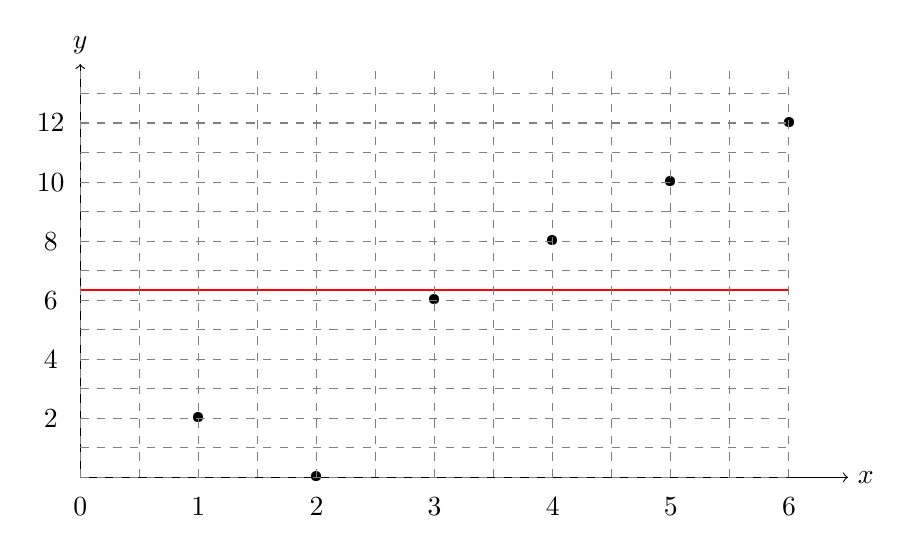
\begin{tikzpicture}[scale = 1.5] \label{regression_trees::plot0}
    % Draw the axes
    \draw[->] (0,0) -- (6.5,0) node[right] {$x$};
    \draw[->] (0,0) -- (0,3.5) node[above] {$y$};

    % Draw points
    \foreach \Point in {(1,0.5), (2,0), (3,1.5), (4,2), (5,2.5), (6,3)}{
        \node at \Point {\textbullet};
    }

    % Draw the piecewise linear function
    \draw[red, thick] (0,38/24) -- (6,38/24);

    % Draw grid lines for better visualization (optional)
    \foreach \x in {0,0.5,1,1.5,2,2.5,3,3.5,4,4.5,5,5.5,6}
        \draw[gray, dashed] (\x,0) -- (\x,3.5);
    \foreach \y in {0,0.25,0.5,0.75,1,1.25,1.5,1.75,2,2.25,2.5,2.75,3,3.25}
        \draw[gray, dashed] (0,\y) -- (6,\y);

    % Axis labels
    \foreach \x in {0,1,2,3,4,5,6}
        \node at (\x,-0.25) {\x};
    \foreach \x in {2,4,6,8,10,12}
        \node at (-0.25,0.25*\x) {\x};

    \end{tikzpicture}
    \end{center}
    
    Вычислим значение метрики для всех возможных разделений объектов на два множества по пороговому значению $x$ в таблице \ref{regression_trees::table1}.
    \begin{table}[h] 
    \centering
    \caption{Вычисление метрики для различных способов разбиения.}
    \begin{tabular}{|c|c|c|c|c|c|}
    \hline
    Диапазон порогового значения & $(1, 2)$ & $(2, 3)$ & $(3, 4)$ & $(4, 5)$ & $(5, 6)$ \\
    \hline
    Пред. для объектов с $x$ меньше порога & $2$ & $1$ & $2.7$ & $4$ & $5.2$ \\
    \hline
    Пред. для объектов с $x$ больше порога & $7.2$ & $9$ & $10$ & $11$ & $12$ \\
    \hline
    MSE для дерева & $84.8$ & $22$ & $26.7$ & $42$ & $68.8$ \\
    \hline
    \end{tabular} \label{regression_trees::table1}
    \end{table}
    
    Таким образом, оптимальное разбиение лежит в диапазоне между $2$ и $3$. Возьмем среднее $2.5$, поскольку это позволит относить объекты к тому подмножеству, которому оно ближе. Изобразим на графике \ref{regression_trees::plot1} новую функцию, задаваемую деревом.
    
    \begin{center}
    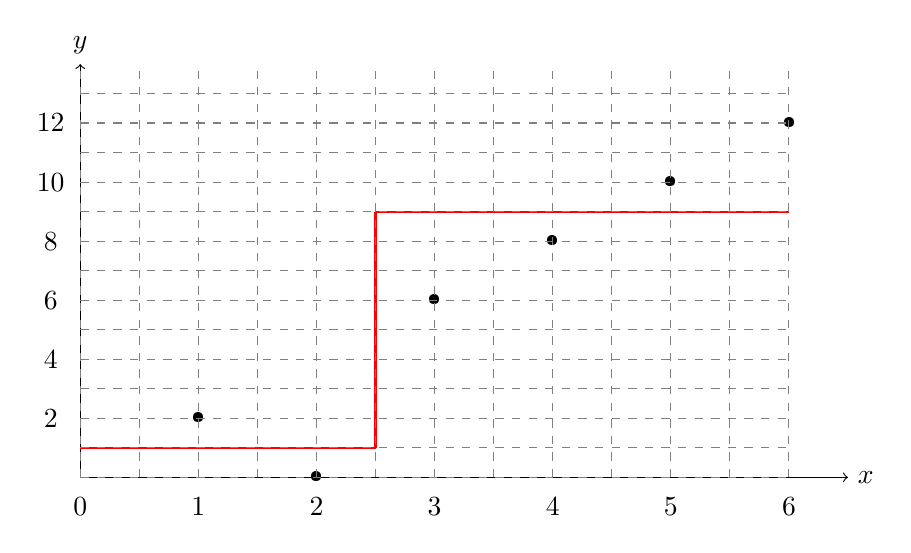
\begin{tikzpicture}[scale = 1.5] 
    % Draw the axes
    \draw[->] (0,0) -- (6.5,0) node[right] {$x$};
    \draw[->] (0,0) -- (0,3.5) node[above] {$y$};

    % Draw points
    \foreach \Point in {(1,0.5), (2,0), (3,1.5), (4,2), (5,2.5), (6,3)}{
        \node at \Point {\textbullet};
    }

    % Draw the piecewise linear function
    \draw[red, thick] (0,0.25) -- (2.5,0.25);
    \draw[red, thick] (2.5,0.25) -- (2.5,2.25);
    \draw[red, thick] (2.5,2.25) -- (6,2.25);

    % Draw grid lines for better visualization (optional)
    \foreach \x in {0,0.5,1,1.5,2,2.5,3,3.5,4,4.5,5,5.5,6}
        \draw[gray, dashed] (\x,0) -- (\x,3.5);
    \foreach \y in {0,0.25,0.5,0.75,1,1.25,1.5,1.75,2,2.25,2.5,2.75,3,3.25}
        \draw[gray, dashed] (0,\y) -- (6,\y);

    % Axis labels
    \foreach \x in {0,1,2,3,4,5,6}
        \node at (\x,-0.25) {\x};
    \foreach \x in {2,4,6,8,10,12}
        \node at (-0.25,0.25*\x) {\x};

    \end{tikzpicture}
    \label{regression_trees::plot1}
    \end{center}

    Проведем разветвление для подмножества с большими значениями $x$. Исходное значение MSE для поддерева равно $20$. Вычислим его для всех вариантов разбиения в таблице \ref{regression_trees::table2}.
    \begin{table}[h] 
    \centering
    \caption{Вычисление метрики для различных способов разбиения.}
    \begin{tabular}{|c|c|c|c|} 
    \hline
    Диапазон порогового значения & $(3, 4)$ & $(4, 5)$ & $(5, 6)$ \\
    \hline
    Пред. для объектов с $x$ меньше порога & $6$ & $7$ & $8$ \\
    \hline
    Пред. для объектов с $x$ больше порога & $10$ & $11$ & $12$ \\
    \hline
    MSE для дерева & $8$ & $4$ & $8$ \\
    \hline
    \end{tabular}
    \label{regression_trees::table2}
    \end{table}

    Таким образом, эффективнее поставить границу между $4$ и $5$, аналогично возьмем среднее $4.5$.

    Оба разбиения достаточно хороши и превосходят результат для поддерева без разбиения ($8$). Выберем первое из них, положив границу $4.5$. Новый график - \ref{regression_trees::plot2}. Левым поддеревом будем называть то поддерево, которое работает с множеством левее по оси $x$.

    \begin{center}
    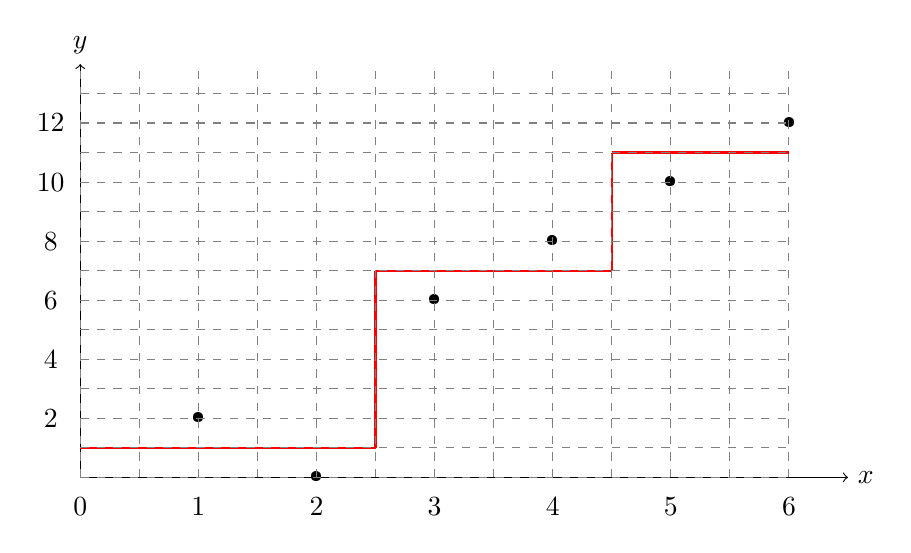
\begin{tikzpicture}[scale = 1.5] \label{regression_trees::plot2}
    % Draw the axes
    \draw[->] (0,0) -- (6.5,0) node[right] {$x$};
    \draw[->] (0,0) -- (0,3.5) node[above] {$y$};

    % Draw points
    \foreach \Point in {(1,0.5), (2,0), (3,1.5), (4,2), (5,2.5), (6,3)}{
        \node at \Point {\textbullet};
    }

    % Draw the piecewise linear function
    \draw[red, thick] (0,0.25) -- (2.5,0.25);
    \draw[red, thick] (2.5,0.25) -- (2.5,1.75);
    \draw[red, thick] (2.5,1.75) -- (4.5,1.75);
    \draw[red, thick] (4.5,1.75) -- (4.5,2.75);
    \draw[red, thick] (4.5,2.75) -- (6,2.75);

    % Draw grid lines for better visualization (optional)
    \foreach \x in {0,0.5,1,1.5,2,2.5,3,3.5,4,4.5,5,5.5,6}
        \draw[gray, dashed] (\x,0) -- (\x,3.5);
    \foreach \y in {0,0.25,0.5,0.75,1,1.25,1.5,1.75,2,2.25,2.5,2.75,3,3.25}
        \draw[gray, dashed] (0,\y) -- (6,\y);

    % Axis labels
    \foreach \x in {0,1,2,3,4,5,6}
        \node at (\x,-0.25) {\x};
    \foreach \x in {2,4,6,8,10,12}
        \node at (-0.25,0.25*\x) {\x};

    \end{tikzpicture}
    \end{center}

    Далее можно провести разбиение трех получившихся множеств, разделяя их посередине между значениями $x$, и присваивая листьям значения $y$ соответствующих $x$. Это уменьшит значение MSE всего дерева до нуля. Изобразим итоговую функцию на графике \ref{regression_trees::plot3}.

    \begin{center}
    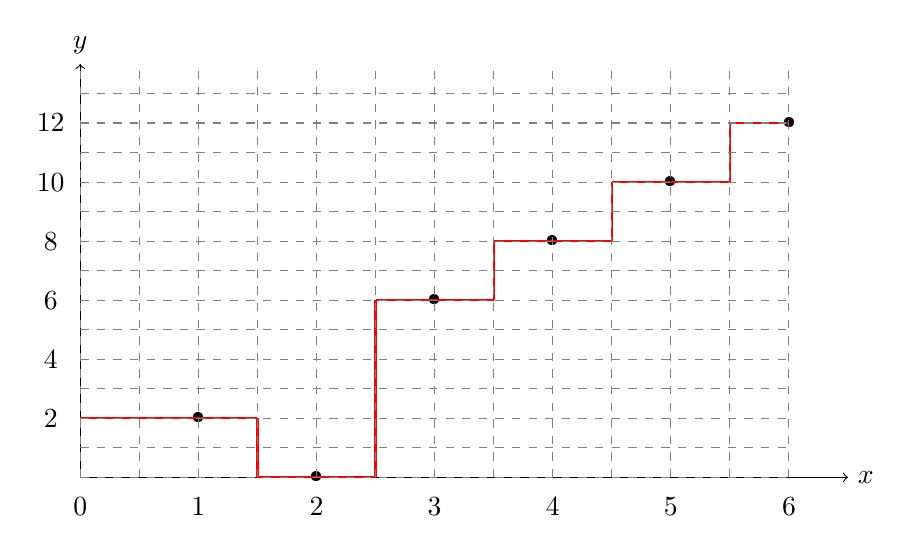
\begin{tikzpicture}[scale = 1.5] \label{regression_trees::plot3}
    % Draw the axes
    \draw[->] (0,0) -- (6.5,0) node[right] {$x$};
    \draw[->] (0,0) -- (0,3.5) node[above] {$y$};

    % Draw points
    \foreach \Point in {(1,0.5), (2,0), (3,1.5), (4,2), (5,2.5), (6,3)}{
        \node at \Point {\textbullet};
    }

    % Draw the piecewise linear function
    \draw[red, thick] (0,0.5) -- (1.5,0.5);
    \draw[red, thick] (1.5,0) -- (2.5,0);
    \draw[red, thick] (2.5,1.5) -- (3.5,1.5);
    \draw[red, thick] (3.5,2) -- (4.5,2);
    \draw[red, thick] (4.5,2.5) -- (5.5,2.5);
    \draw[red, thick] (5.5,3) -- (6,3);
    
    \draw[red, thick] (1.5,0) -- (1.5,0.5);
    \draw[red, thick] (2.5,0) -- (2.5,1.5);
    \draw[red, thick] (3.5,1.5) -- (3.5,2);
    \draw[red, thick] (4.5,2) -- (4.5,2.5);
    \draw[red, thick] (5.5,2.5) -- (5.5,3);

    % Draw grid lines for better visualization (optional)
    \foreach \x in {0,0.5,1,1.5,2,2.5,3,3.5,4,4.5,5,5.5,6}
        \draw[gray, dashed] (\x,0) -- (\x,3.5);
    \foreach \y in {0,0.25,0.5,0.75,1,1.25,1.5,1.75,2,2.25,2.5,2.75,3,3.25}
        \draw[gray, dashed] (0,\y) -- (6,\y);

    % Axis labels
    \foreach \x in {0,1,2,3,4,5,6}
        \node at (\x,-0.25) {\x};
    \foreach \x in {2,4,6,8,10,12}
        \node at (-0.25,0.25*\x) {\x};

    \end{tikzpicture}
    \end{center}
    
\textbf{Задача 3} (Усечение решающего дерева)
    
    Проведите отсечение ветвей дерева, полученнного в предыдущей задаче с использованием выборки: 
    \begin{table}[h]
    \centering
    \caption{Выборка.}
    \begin{tabular}{|c|c|c|c|c|c|}
    \hline
    $x$ & $1.25$ & $2.25$ & $3.25$ & $4.25$ & $5.25$ \\
    \hline
    $y$ & $2.5$ & $4.5$ & $6.5$ & $8.5$ & $10.5$ \\
    \hline
    \end{tabular}
    \end{table}
    Проанализируйте полученные результаты.

    \textbf{Решение.}
    Изобразим на графике новые точки:

    \begin{center}
    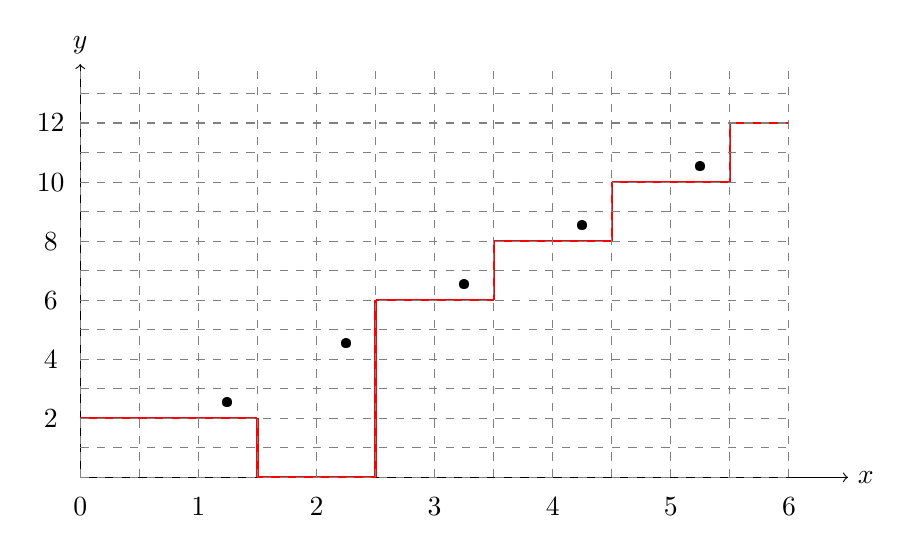
\begin{tikzpicture}[scale = 1.5] \label{regression_trees::plot4}
    % Draw the axes
    \draw[->] (0,0) -- (6.5,0) node[right] {$x$};
    \draw[->] (0,0) -- (0,3.5) node[above] {$y$};

    % Draw points
    \foreach \Point in {(1.25,0.625), (2.25,1.125), (3.25,1.625), (4.25,2.125), (5.25,2.625)}{
        \node at \Point {\textbullet};
    }

    % Draw the piecewise linear function
    \draw[red, thick] (0,0.5) -- (1.5,0.5);
    \draw[red, thick] (1.5,0) -- (2.5,0);
    \draw[red, thick] (2.5,1.5) -- (3.5,1.5);
    \draw[red, thick] (3.5,2) -- (4.5,2);
    \draw[red, thick] (4.5,2.5) -- (5.5,2.5);
    \draw[red, thick] (5.5,3) -- (6,3);
    
    \draw[red, thick] (1.5,0) -- (1.5,0.5);
    \draw[red, thick] (2.5,0) -- (2.5,1.5);
    \draw[red, thick] (3.5,1.5) -- (3.5,2);
    \draw[red, thick] (4.5,2) -- (4.5,2.5);
    \draw[red, thick] (5.5,2.5) -- (5.5,3);

    % Draw grid lines for better visualization (optional)
    \foreach \x in {0,0.5,1,1.5,2,2.5,3,3.5,4,4.5,5,5.5,6}
        \draw[gray, dashed] (\x,0) -- (\x,3.5);
    \foreach \y in {0,0.25,0.5,0.75,1,1.25,1.5,1.75,2,2.25,2.5,2.75,3,3.25}
        \draw[gray, dashed] (0,\y) -- (6,\y);

    % Axis labels
    \foreach \x in {0,1,2,3,4,5,6}
        \node at (\x,-0.25) {\x};
    \foreach \x in {2,4,6,8,10,12}
        \node at (-0.25,0.25*\x) {\x};

    \end{tikzpicture}
    \end{center}

    Проведем усечение снизу-вверх, анализируя сначала меньшие поддеревья, и будем объединять узлы там, где это улучшает результат. Это стратегия Reduced Error Pruning.
    
    Проанализируем все поддеревья, имеющие два листа. Это диапазоны $(1, 2.5)$, $(2.5, 4.5)$ и $(4.5, 6)$. Вычислим для них MSE при текущих предсказаниях и при объединении листьев обратно в одну ноду. Отразим результаты в таблице \ref{regression_trees::table3}.

    \begin{table}[h] 
    \centering
    \caption{Вычисление метрики для различных способов разбиения.}
    \begin{tabular}{|c|c|c|c|} 
    \hline
    Поддерево & $(1, 2.5)$ & $(2.5, 4.5)$ & $(4.5, 6)$ \\
    \hline
    MSE исходно & $18.125$ & $0.125$ & $0.125$ \\
    \hline
    MSE объединения & $12.125$ & $2.125$ & $2.125$ \\
    \hline
    MSE с предсказанием левого поддерева & $5.125$ & $5.125$ & $3.125$ \\
    \hline
    MSE с предсказанием правого поддерева & $23.125$ & $5.125$ & $3.125$ \\
    \hline
    \end{tabular}
    \label{regression_trees::table3}
    \end{table}

    Таким образом, в поддереве $(1, 2.5)$ разделение неэффективно, и лучше заменить его на левое поддерево. Для остальных же вершин разделение должно остаться. Изобразим новое дерево на графике \ref{regression_trees::plot5}.
    
    \begin{center}
    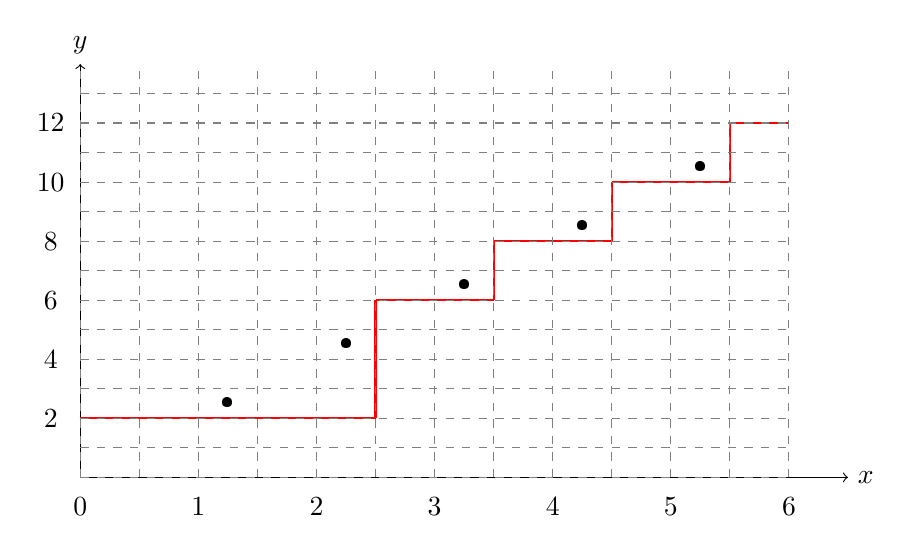
\begin{tikzpicture}[scale = 1.5] \label{regression_trees::plot5}
    % Draw the axes
    \draw[->] (0,0) -- (6.5,0) node[right] {$x$};
    \draw[->] (0,0) -- (0,3.5) node[above] {$y$};

    % Draw points
    \foreach \Point in {(1.25,0.625), (2.25,1.125), (3.25,1.625), (4.25,2.125), (5.25,2.625)}{
        \node at \Point {\textbullet};
    }

    % Draw the piecewise linear function
    \draw[red, thick] (0,0.5) -- (2.5,0.5);
    \draw[red, thick] (2.5,1.5) -- (3.5,1.5);
    \draw[red, thick] (3.5,2) -- (4.5,2);
    \draw[red, thick] (4.5,2.5) -- (5.5,2.5);
    \draw[red, thick] (5.5,3) -- (6,3);
    
    \draw[red, thick] (2.5,0.5) -- (2.5,1.5);
    \draw[red, thick] (3.5,1.5) -- (3.5,2);
    \draw[red, thick] (4.5,2) -- (4.5,2.5);
    \draw[red, thick] (5.5,2.5) -- (5.5,3);

    % Draw grid lines for better visualization (optional)
    \foreach \x in {0,0.5,1,1.5,2,2.5,3,3.5,4,4.5,5,5.5,6}
        \draw[gray, dashed] (\x,0) -- (\x,3.5);
    \foreach \y in {0,0.25,0.5,0.75,1,1.25,1.5,1.75,2,2.25,2.5,2.75,3,3.25}
        \draw[gray, dashed] (0,\y) -- (6,\y);

    % Axis labels
    \foreach \x in {0,1,2,3,4,5,6}
        \node at (\x,-0.25) {\x};
    \foreach \x in {2,4,6,8,10,12}
        \node at (-0.25,0.25*\x) {\x};

    \end{tikzpicture}
    \end{center}    

    Проведя аналогичные вычисления для поддеревьев $(2.5, 6)$ и $(1, 6)$ получим, что другие объединения не улучшают результат. Таким образом, усечение завершено.

    \textbf{Анализ результатов.} Если посмотреть на две выборки вместе, то график напоминает линейную зависимость, в которой точка $(2, 0)$ является выбросом. Таким образом, эти две задачи иллюстрируют склонность деревьев переобучаться на выбросах. Усечение ветвей позволяет компенсировать выбросы и устранять переобучение, усредняя значение с соседними точками, или заменяя всё поддерево на поддерево их анализа. 


\section{Небрежные решающие деревья}

\subsection{Общее описание}

\textbf{Небрежное решающее дерево} (oblivious decision tree, ODT, решающая таблица) --- решающее дерево глубины $H$,
у которого на любом уровне $h < H$ условие ветвления $f_h(x)$ одинаково для всех вершин этого уровня, и на 
уровне $h$ ровно $2^{h-1}$ вершин.

Таким образом все пространство делится на $2^H$ ячеек. Метод также называется решающей таблицей, потому что классификатор
задается таблицей с $2^H$ ячейками:
\begin{equation*}
    T: \{0, 1\}^H \rightarrow Y: a(x) = T(f_1(x), ..., f_H(x))
\end{equation*}

Отметим, что в данной постановке у каждой внутренней вершины решающего дерева будет ровно $2$ дочерних вершины. На самом деле,
их не обязательно должно быть именно $2$, главное, чтобы у всех внутренних вершин было одинаковое количество дочерних.

\subsection{Преимущества ODT}
\begin{itemize}
    \item Интерпретация как решающей таблицы дает тривиальную реализацию с низкой вычислительной сложностью
    \item Жесткая структура дерева избавляет от проблем с переобучением и сложностью интерпретации модели
\end{itemize}

\subsection{Недостатки ODT}
\begin{itemize}
    \item Модель почти всегда будет весьма грубой и неточной из-за строго заданной структуры дерева
\end{itemize}

\subsection{Обучение}

Разберемся, как обучать такую модель. Поскольку это все еще решающее дерево, модифицируем алгоритм ID3 так, чтобы построенное
дерево удовлетворяло было небрежным решающим деревом. Условия ветвления одинаковы в рамках одного уровня, поэтому модификация
ID3 не будет рекурсивной, а будет итеративно строить каждый слой сразу.

\begin{algorithm}
\caption{Алгоритм обучения ODT}\label{alg:cap}
\hspace*{\algorithmicindent} \textbf{Вход:} выборка $X^{\ell}$; множество признаков $F$; глубина дерева $H$ \\ 
\hspace*{\algorithmicindent} \textbf{Выход:} признаки $f_h \; \forall h=1,...,H$, таблица $T: \{0, 1\}^H \rightarrow Y$
\begin{algorithmic}
    \For{$h=1,...,H$}
        \State \texttt{Найдем предикат, дающий максимальное увеличение определенности}
        \State $ f_h \gets \text{argmax}_{f \in F} Gain(f_1, ..., f_{h-1}, f)$
    \EndFor
    \State \texttt{Установим класс по мажоритарному правилу}
    \State $ T(\beta) \gets Major(U_{H\beta}) \quad \forall \beta \in \{0, 1\}^H$
\end{algorithmic}
\end{algorithm}

Увеличение определенности считается следующим образом:
\begin{equation*}
    Gain(f_1, ..., f_h) = \Phi(X^{\ell}) - \sum\limits_{\beta\in \{0, 1\}^h}\frac{U_{h\beta}}{\ell}\Phi(U_{h\beta}) 
\end{equation*}
\begin{equation*}
    U_{h\beta} = \{x_i\in X^{\ell}: f_s(x_i)=\beta_s, \; s=1,...,h\}, \beta=(\beta_1, ...,\beta_h)\in\{0, 1\}^h
\end{equation*}

\subsection{Задачи}

\textbf{Задача 1}

Постройте небрежное решающее дерево для задачи XOR.

\textbf{Решение}

$ x = (\xi_1, \xi_2) $, где $ \xi_1, \xi_2\in(-1, 1) $.
Нужно предсказывать значение предиката <<$\xi_1$ и $\xi_2$ разного знака>>.

Представим решение в виде решающей таблицы: \\
$H = 2$ \\
$ f_i(x) = \mathbb{I}(\xi_i > 0), \; i = 1, 2 $. \\
$T(0, 0) = T(1, 1) = 0$ \\
$T(0, 1) = T(1, 0) = 1$

\textbf{Задача 2}

Почему небрежные решающие деревья хорошо подходят для использования в ансамблях моделей?

\textbf{Решение}

Потому что они легко обучаются и вычисляются,
однако при этом предоставляют достаточно хорошую точность (для настолько легких моделей), потому что все еще являются
решающими деревьями.

\textbf{Задача 3}

Чувствительны ли небрежные решающие деревья к шумам в данных?

\textbf{Решение}

Не очень чувствительны, потому что необходимость выбирать общий критерий для всех ветвей сразу не дает возможности
модели подстроиться под малые изменения данных. Поэтому при добавлении некоторого шума к обучающей выборке построенное
небрежное решающее дерево изменится незначительно.

\subsection*{Алгоритм бустинга}

Алгоритмы КОРА и ТЭМП имеют общий недостаток~--- они не стремятся увеличивать различность комбинаций. Эта проблема решается в алгоритме бустинга.

\textit{Бустинг} (boosting) предложили американские учёные Фройнд и Шапир как универсальный метод построения выпускной комбинации классификаторов. 

В бустинге закономерности строятся последовательно, и после построения очередной закономерности веса выделенных ею объектов изменяются~--- уменьшаются у позитивных и увеличиваются у негативных объектов. Обновлённый вектор весов $w$ у объектов $x$ определяется следующей закономерностью по критерию максимума \textit{взвешенной информации}. В результате каждая следующая закономерность стремится выделять ``наименее покрытые'' объекты, оказывающиеся ``наиболее трудными'' для предыдущих закономерностей. Это способ повышения разнообразия закономерностей, более равномерного покрытия объектов и повышения обобщающей способности выпускной комбинации закономерностей.

Описанная стратегия напоминает алгоритм построения решающего списка. Разница в том, что там было достаточно покрыть объект один раз, после чего он исключался из рассмотрения. Здесь же каждое покрытие только изменяет вес объекта.

Для реализации этой идеи остаётся понять, как именно должны изменяться веса объектов и веса закономерностей на каждом этапе алгоритма.

Рассмотрим задачу классификации с двумя классами, $Y = \{-1, +1\}$ и алгоритм взвешенного голосования, состоящий из $T = T_{-1} + T_{+1}$ закономерностей:
\begin{equation}
    a_T(x) = \text{sign}\left( \sum_{t=1}^{T_{+1}} \alpha^t_{+1} \varphi^t_{+1}(x) - \sum_{t=1}^{T_{-1}} \alpha^t_{-1} \varphi^t_{-1}(x) \right), \quad \alpha^t_c > 0, \, c \in Y.
\end{equation}

\subsection*{Экспоненциальная аппроксимация пороговой функции потерь}

Пусть уже построено $T$ закономерностей, вместе составляющих алгоритм классификации $a_T(x)$. При добавлении ещё одной закономерности $\varphi_c(x)$ в список $\mathcal{R}_c$ взвешенная сумма голосов за класс $c \in \{-1, +1\}$ примет вид
\begin{equation}
    \Gamma'_c(x) = \Gamma_c(x) + \alpha \varphi_c(x).
\end{equation}

Задача состоит в том, чтобы найти закономерность $\varphi_c$ и её вес $\alpha$, при которых алгоритм $a_{T+1}(x)$ допускает минимальное число ошибок на обучающей выборке $X^\ell$.

Число ошибок алгоритма $a_T(x)$ перед добавлением закономерности $\varphi_c$:
\begin{equation}
    Q_T = \sum_{i=1}^\ell \left[ \Gamma_{y_i}(x_i) - \Gamma_{-y_i}(x_i) < 0 \right].
\end{equation}

Число ошибок алгоритма $a_{T+1}(x)$ после добавления закономерности $\varphi_c$:
\begin{equation}
    Q_{T+1}(\varphi_c, \alpha) = \sum_{i=1}^\ell \left[ y_i = c \right] 
    \left[ \Gamma_{y_i}(x_i) - \Gamma_{-y_i}(x_i) + \alpha \varphi_c(x_i) < 0 \right] + 
    \sum_{i=1}^\ell \left[ y_i \neq c \right] 
    \left[ \Gamma_{y_i}(x_i) - \Gamma_{-y_i}(x_i) + \alpha \varphi_c(x_i) < 0 \right].
\end{equation}

Выписанный функционал содержит параметр $\alpha$ внутри пороговой функции вида $\left[ z(\alpha) < 0 \right]$, следовательно, является разрывной функцией от $\alpha$. Минимизация такого функционала является нетривиальной задачей комбинаторной оптимизации. Попробуем упростить её приближением. Заменим пороговую функцию непрерывно дифференцируемой оценкой сверху. Тогда минимизацию по $\alpha$ можно будет выполнить аналитически.

Запишем верхнюю оценку $\tilde{Q}_T$ функционала $Q_T$:
\begin{equation}
    Q_T \leq \tilde{Q}_T \equiv \sum_{i=1}^\ell \exp\left(\Gamma_{-y_i}(x_i) - \Gamma_{y_i}(x_i)\right) = \sum_{i=1}^\ell w_i.
\end{equation}

Если алгоритм $a_T(x)$ правильно классифицирует объект $x_i$, то $w_i < 1$. Если ошибается, то $w_i > 1$. Чем больше перевес голосов в пользу ошибочного класса, тем больше вес $w_i$. Таким образом, большие веса получают наиболее ``трудные'' объекты.

Введём вектор весов $w = \{w_i\}_{i=1}^\ell$ с компонентами $w_i = \ell \tilde{w}_i / \tilde{Q}_T$. Тогда будет выполнено условие нормировки $\sum_{i=1}^\ell w_i = \ell$. Следующая теорема показывает, что выбор $w_i$ в качестве весов объектов оптимален для построения $(T+1)$-й закономерности.

\textbf{Теорема 1.2.} Минимум функционала $\tilde{Q}_{T+1}(\varphi_c, \alpha)$ достигается при
\begin{equation}
    \varphi_c^* = \arg \max_{\varphi_c \in \mathcal{R}_c} J_c^w(\varphi_c, X^\ell), \quad
    J_c^w(\varphi_c, X^\ell) = \sqrt{p_c^w(\varphi_c)} - \sqrt{n_c^w(\varphi_c)},
\end{equation}
\begin{equation}
    \alpha^* = \frac{1}{2} \ln \frac{p_c^w(\varphi_c^*)}{n_c^w(\varphi_c^*)}, \quad \text{при } n_c^w(\varphi_c) \neq 0,
\end{equation}
где функции $p_c^w$ и $n_c^w$ определяются по формулам (1.3).

\textbf{Доказательство.} 

Распишем функционал $\tilde{Q}_{T+1}$, воспользовавшись тождеством $e^A = (1-\varphi) + \varphi e^A$, которое справедливо при любых $A \in \mathbb{R}$ и $\varphi \in \{0,1\}$.

\begin{equation}
    \tilde{Q}_{T+1} = \sum_{i=1}^\ell w_i e^{-\alpha \varphi_c(x_i)} \left[ y_i = c \right] 
    + \sum_{i=1}^\ell w_i e^{\alpha \varphi_c(x_i)} \left[ y_i \neq c \right] =
    \sum_{i=1}^\ell w_i (1 - \varphi_c(x_i)) + e^{-\alpha} \sum_{i=1}^\ell w_i \varphi_c(x_i) \left[ y_i = c \right] 
    + e^\alpha \sum_{i=1}^\ell w_i \varphi_c(x_i) \left[ y_i \neq c \right].
\end{equation}

Подставим в эту формулу $w_i = \tilde{w}_i \tilde{Q}_T / \ell$ и обозначим для краткости $p = p_c^w(\varphi_c)$, $n = n_c^w(\varphi_c)$. Тогда, согласно определению (1.3),
\begin{equation}
    \tilde{Q}_{T+1} = \frac{\tilde{Q}_T}{\ell} \left( \sum_{i=1}^\ell \tilde{w}_i - \sum_{i=1}^\ell \tilde{w}_i \varphi_c(x_i) + e^{-\alpha} \sum_{i \colon y_i = c} \tilde{w}_i \varphi_c(x_i) + e^\alpha \sum_{i \colon y_i \neq c} \tilde{w}_i \varphi_c(x_i) \right) = 
    \frac{\tilde{Q}_T}{\ell} \left( \ell - p - n + e^{-\alpha} p + e^\alpha n \right).
    \label{eq:q_tilde}
\end{equation}

Минимум этого выражения по $\alpha$ достигается при $e^{-\alpha} = e^\alpha n / p$, откуда вытекает 
\begin{equation}
    \alpha^* = \frac{1}{2} \ln \frac{p}{n}, \quad \text{если только } n \neq 0.
\end{equation}

Подставляя $\alpha^*$ в функционал $\tilde{Q}_{T+1}$, получаем:
\begin{equation}
    \tilde{Q}_{T+1} = \frac{\tilde{Q}_T}{\ell} \left( \ell - p - n + 2 \sqrt{p n} \right) = \tilde{Q}_T \left( 1 - \frac{1}{\ell} \left( \sqrt{p} - \sqrt{n} \right)^2 \right).
\end{equation}

Минимизация этого функционала по предикату $\varphi_c$ эквивалентна максимизации функционала $J_c^w(\varphi_c) = \sqrt{p} - \sqrt{n}$ по $\varphi_c$, что и требовалось доказать.

\subsection*{Замечание 1.5}

Теорема не позволяет определить вес непроверяющей закономерности $\varphi_c^*$, так как знаменатель (1.11) обращается в нуль. Это происходит потому, что, согласно (1.12), при $n = 0$ функционал $\tilde{Q}_{T+1}$ неограниченно убывает по $\alpha$, и непроверяющие закономерности бесконечно выгодны с точки зрения минимизации $\tilde{Q}_{T+1}$. Чтобы предотвратить этот нежелательный эффект, вводят дополнительный параметр $\lambda \in (0, 1)$, слегка модифицируя формулу расчёта веса:
\begin{equation}
    \alpha^* = \frac{1}{2} \ln \frac{p_c^w(\varphi_c^*)}{\max\{n_c^w(\varphi_c^*), \lambda\}}.
\end{equation}

Это всё равно, что ввести в функционал $\tilde{Q}_{T+1}$ дополнительное штрафное слагаемое с коэффициентом $\lambda$:
\begin{equation}
    \tilde{Q}_{T+1} \equiv \tilde{Q}_T \left( \ell - p - n + e^{-\alpha} p + e^\alpha n + \lambda e^\alpha \left[ n = 0 \right] \right).
\end{equation}

Чем меньше $\lambda$, тем больший вес получают непроверяющие закономерности. Таким образом, управляя параметром $\lambda$, можно заставить алгоритм искать преимущественно непроверяющие закономерности.

\textbf{Алгоритм 1.10.} Построение выпускной комбинации закономерностей при классификации на два класса, $Y = \{-1, +1\}$ (алгоритм бустинга).

\textbf{Вход:}
\begin{itemize}
    \item $X^\ell$~--- обучающая выборка;
    \item $\Phi$~--- семейство базовых предикатов;
    \item $T$~--- общее число закономерностей всех классов;
    \item $\lambda$~--- коэффициент поощрения непроверяющих закономерностей.
\end{itemize}

\textbf{Выход:} списки закономерностей и их весов $\{ \varphi_c^t(x), \alpha_c^t \mid t = 1, \ldots, T_c \}$ для всех $c \in Y$.

\begin{enumerate}
    \item Инициализировать веса: $w_i = 1$ для всех $i = 1, \ldots, \ell$;
    \item \textbf{для} всех $t = 1, \ldots, T$:
    \begin{enumerate}
        \item $c = c_t$~--- выбрать класс, для которого будет строиться закономерность;
        \item $\varphi_c^t = \arg\max_{\varphi \in \Phi} \sqrt{p_c^w(\varphi)} - \sqrt{n_c^w(\varphi)}$;
        \item $\alpha_c^t = \frac{1}{2} \ln \frac{p_c^w(\varphi_c^t)}{\max\{n_c^w(\varphi_c^t), \lambda\}}$;
        \item \textbf{для всех} $i = 1, \ldots, \ell$ пересчитать веса $w_i$:
        \[
            w_i' =
            \begin{cases}
                w_i, & \varphi_c^t(x_i) = 0; \\
                w_i e^{-\alpha_c^t}, & \varphi_c^t(x_i) = 1 \text{ и } y_i = c; \\
                w_i e^{\alpha_c^t}, & \varphi_c^t(x_i) = 1 \text{ и } y_i \neq c;
            \end{cases}
        \]
        \item нормировать веса: $w_i = w_i' / Z$ для всех $i = 1, \ldots, \ell$;
    \end{enumerate}
\end{enumerate}

\textbf{Замечание 1.6.} После того, как закономерность $\varphi_c(x)$ найдена и вычислен соответствующий ей коэффициент $\alpha$, легко пересчитать веса объектов $w_i'$ для следующего шага алгоритма:
\[
    w_i' = w_i \left( \left[ y_i = c \right] e^{-\alpha_c(x_i)} + \left[ y_i \neq c \right] e^{\alpha_c(x_i)} \right).
\]
Таким образом, при выделении позитивного объекта его вес уменьшается в $e^\alpha$ раз, а при выделении негативного~--- увеличивается во столько же раз. В результате многократного применения этого правила бустинг стремится выделять позитивные объекты ``равномерно часто'', а негативные~--- ``равномерно редко''.

\textbf{Замечание 1.7.} Фактически, теорема 1.2 вводит ещё один функционал информации предикатов $J_c^w(\varphi) = \sqrt{p_c^w(\varphi)} - \sqrt{n_c^w(\varphi)}$. Как видно из таблицы 1, он достаточно адекватно оценивает качество закономерностей, а вычисляется существенно проще, чем $I_c^w(\varphi)$. Его можно применять не только в алгоритме бустинга, но и отдельно, поскольку теорема 1.2 остаётся верна для функционала $\tilde{Q}_T$, если учитывать все веса $w_i$ равными единице.

\textbf{Замечание 1.8.} В процессе работы алгоритма имеет смысл проанализировать распределение весов объектов. Объекты с наибольшими весами $w_i$ являются наиболее ``трудными'' для классификации.

``Трудными'' для всех построенных закономерностей. Возможно, это ``шумовые выбросы''~--- объекты, в описании которых допущены грубые ошибки. Исключение таких объектов, называемое \textit{цензурированием выборки}, как правило, повышает качество классификации. После исключения выбросов построение закономерностей лучше начать заново, поскольку выбросы мешали адекватно оценивать информативность закономерностей.

\subsection*{Замечание 1.9}
В Алгоритме \textbf{1.10} основная работа выполняется на шаге 4, когда ищется закономерность, доставляющая максимальное значение функционалу информативности $J_c^w(\varphi)$. Для решения данной задачи можно воспользоваться любым доступным алгоритмом синтеза закономерностей~--- градиентным, генетическим, TEMPO и модификациями $T_0 = 1$, и т.д. Единственное ограничение, которое для этого требуется~--- заменить критерий информативности $I_c$ на $J_c^w$. Отметим, что симбиоз ``бустинг + ТЭМП с редукцией правил'' практически совпадает с алгоритмом SLIPPER (simple learner with iterative pruning to produce error reduction), который считается одним из лучших логических алгоритмов классификации.

\subsection*{Теорема сходимости}
Бустинг гарантирует построение корректного алгоритма, не допускающего ошибок на обучающей выборке. Оказывается, для этого достаточно потребовать, чтобы на шаге 4 всякий раз удавалось найти закономерность $\varphi_c^t$ со строго положительной информативностью $J_c^w(\varphi_c^t)$.

\subsection*{Теорема 1.3}
Для числа ошибок на обучении справедлива оценка:
\begin{equation}
    Q_T \leq \ell \prod_{t=1}^T \left( 1 - \frac{J_t^2}{\ell} \right), \quad \text{где} \quad J_t = \sqrt{p_c^w(\varphi_c^t)} - \sqrt{n_c^w(\varphi_c^t)}.
    \label{eq:convergence}
\end{equation}

Если на каждом шаге алгоритма бустинга находится закономерность $\varphi_c^t$ с информативностью $J_t > J > 0$, то для обращения функционала $Q_T$ в нуль потребуется не более $T_0 = (\ell \ln \ell) / J^2$ шагов.

\subsection*{Доказательство}
При доказательстве теоремы \textbf{1.2} была получена рекуррентная формула:
\begin{equation}
    \tilde{Q}_{t+1} = \tilde{Q}_t \left( 1 - \frac{J_t^2}{\ell} \right).
\end{equation}

Аналогично доказывается, что на первом шаге алгоритма, когда веса $w_i$ единичны,
\[
    \tilde{Q}_1 = \ell \left( 1 - \frac{J_1^2}{\ell} \right).
\]

Поскольку $Q_T \leq \tilde{Q}_T$, отсюда немедленно вытекает~\eqref{eq:convergence}. Для доказательства сходимости за конечное число шагов оценим $Q_T$ сверху:
\[
    Q_T \leq \ell \prod_{t=1}^T \left( 1 - \frac{J^2}{\ell} \right)^T \leq \ell \exp\left( -\frac{J^2 T}{\ell} \right).
\]

При $T > T_0$ эта оценка становится меньше $1$ и функционал $Q_T$ обращается в нуль, поскольку он может принимать только целые неотрицательные значения. \hfill $\blacksquare$

\subsection*{Достоинства бустинга.}

\begin{itemize}
    \item \textbf{Высокая обобщающая способность} достигается за счёт более равномерного покрытия объектов закономерностями.

    \item \textbf{Корректность на обучающей выборке} гарантируется при достаточно слабых дополнительных ограничениях.

    \item \textbf{Универсальность.} Можно использовать любое семейство базовых предикатов $\Phi$, не обязательно конъюнкции. Предполагается только, что на шаге 4 применяется достаточно эффективный алгоритм перебора по множеству $\Phi$.

    \item \textbf{Эффективность} бустинга целиком определяется этим внешним алгоритмом. Собственные накладные расходы бустинга невелики.

    \item \textbf{Интерпретируемость.} Линейная комбинация правил легко интерпретируется, если правил немного и они имеют вид конъюнкций. Веса правил всегда положительны и показывают степень их важности для классификации.

    \item \textbf{Фильтрация шума.} Возможность выделения шумовых объектов.
\end{itemize}

\subsection*{Недостатки бустинга.}

\begin{itemize}
    \item \textbf{Эффект переобучения} может всё же наблюдаться, если на шаге 4 не удаётся находить достаточно хорошие закономерности.

    \item В этом случае резко возрастает число правил $T$, необходимых для обеспечения корректности и линейная комбинация теряет свойство интерпретируемости. Алгоритм голосования становится ``чёрным ящиком'' с неочевидной внутренней логикой, когда число правил превышает несколько десятков.
\end{itemize}

\subsection{Задачи}

\textbf{Задача 1}  
Рассмотрим множество элементарных предикатов \( B = \{ \beta_1, \beta_2, \beta_3 \} \) и обучающую выборку \( X_\ell \) с классами \( Y = \{-1, +1\} \). Предположим, что следующие конъюнкции дают прирост взвешенной информативности \( J_w(\varphi) \):

\[
\varphi_1 = \beta_1 \wedge \beta_2, \quad J_w(\varphi_1) = 0.3; \quad
\varphi_2 = \beta_2 \wedge \beta_3, \quad J_w(\varphi_2) = 0.1; \quad
\varphi_3 = \beta_1 \wedge \beta_3, \quad J_w(\varphi_3) = 0.4
\]

Алгоритм бустинга требует, чтобы \( J_w(\varphi) > 0.2 \) для добавления закономерности в итоговый список. Определите, какие из этих конъюнкций будут добавлены в модель на текущем шаге.  

\textbf{Решение}  
Проверяем каждую конъюнкцию:  

\[
\varphi_1: J_w(\varphi_1) = 0.3 > 0.2 \quad \text{(добавляется в модель)},
\]
\[
\varphi_2: J_w(\varphi_2) = 0.1 \leq 0.2 \quad \text{(не добавляется)},
\]
\[
\varphi_3: J_w(\varphi_3) = 0.4 > 0.2 \quad \text{(добавляется в модель)}.
\]

Таким образом, в модель будут добавлены конъюнкции \( \varphi_1 \) и \( \varphi_3 \).

\vspace{0.5cm}

\textbf{Задача 2}  
Предположим, что параметр \( T \) (общее количество правил) в алгоритме бустинга увеличен с 10 до 20. Объясните, как это изменение повлияет на модель.  

\textbf{Решение}  
Увеличение \( T \) с 10 до 20 позволяет алгоритму добавить больше закономерностей в итоговую комбинацию. Это повышает гибкость модели, так как она может лучше подстраиваться под сложные данные. Однако увеличение числа правил может привести к следующим эффектам:
\begin{itemize}
    \item \textbf{Повышение качества на обучающей выборке:} Большее число правил улучшает покрытие объектов, уменьшая количество ошибок на обучении.  
    \item \textbf{Риск переобучения:} Модель может начать подгоняться под шумовые данные, что снизит её обобщающую способность.  
    \item \textbf{Снижение интерпретируемости:} Увеличение числа правил затрудняет анализ и интерпретацию модели.
\end{itemize}

Чтобы избежать переобучения, рекомендуется использовать раннюю остановку или регулировать веса объектов.  

\vspace{0.5cm}

\textbf{Задача 3}  
Предположим, что множество базовых предикатов \( B \) плохо выбрано, и для \( J_w(\varphi) \) многих закономерностей выполняется \( J_w(\varphi) \leq 0.1 \). Как это повлияет на работу алгоритма бустинга, и какие меры можно предпринять для улучшения качества модели?  

\textbf{Решение}  
Если множество предикатов \( B \) плохо выбрано, то алгоритм бустинга не сможет находить закономерности с высокой информативностью, что приведёт к низкому качеству модели. Веса объектов будут перераспределяться неэффективно, и модель не сможет адекватно обобщать данные.  

Для улучшения качества модели можно предпринять следующие меры:
\begin{itemize}
    \item \textbf{Пересмотр множества предикатов:} Добавить новые предикаты, лучше отражающие свойства данных.  
    \item \textbf{Использование более сложных базовых классификаторов:} Например, заменить простые конъюнкции на деревья решений или нейронные сети.  
    \item \textbf{Снижение порога \( J_w(\varphi) > 0.1 \):} Это позволит добавлять в модель больше правил, хотя может повысить риск переобучения.  
    \item \textbf{Анализ ошибок:} Исключить шумовые или аномальные объекты, которые могут мешать выбору информативных закономерностей.
\end{itemize}


\section*{Критерии информативности}

Решающие деревья являются одним из базовых методов машинного обучения, который используется как для задач классификации, так и для задач регрессии. Одним из ключевых аспектов построения эффективных деревьев является выбор критериев, определяющих, насколько информативен тот или иной сплит. Эти критерии играют решающую роль в формировании структуры дерева, определяя его глубину, разбиения и качество предсказаний. 

В данной статье мы рассмотрим популярные подходы к определению информативности сплитов в зависимости от постановки задачи. Мы детально разберем критерии, применяемые в задачах регрессии (среднеквадратичная ошибка, средняя абсолютная ошибка) и классификации (энтропия, критерий Джини и другие).


\subsection*{Информативность в задаче регрессии: MSE}
Посмотрим на простой пример - регрессию с минимизацией среднеквадратичной ошибки:

\[
L\left(y_{i}, c\right)=\left(y_{i}-c\right)^{2}
\]

Информативность листа будет выглядеть следующим образом:

\[
H\left(X_{m}\right)=\frac{1}{\left|X_{m}\right|} \min _{c \in Y} \sum_{\left(x_{i}, y_{i}\right) \in X_{m}}\left(y_{i}-c\right)^{2}
\]

Как мы уже знаем, оптимальным предсказанием константного

классификатора для задачи минимизации MSE является среднее значение, то есть
\[
\(c=\frac{\sum y_{i}}{\left|X_{m}\right|}\)
\]

Подставив в формулу информативности сплита, получаем:
\[
H(X_m) = \sum_{(x_i, y_i) \in X_m} \frac{(y_i - \overline{y})^2}{|X_m|}, \quad \text{где } \overline{y} = \frac{1}{|X_m|} \sum_i y_i
\]

То есть при жадной минимизации MSE информативность - это оценка дисперсии таргетов для объектов, попавших в лист. Получается очень стройная картинка: оценка значения в каждом листе - это среднее, а выбирать сплиты надо так, чтобы сумма дисперсий в листьях была как можно меньше.

\subsection*{Информативность в задаче регрессии: MAE}
\[
\(L\left(y_{i}, c\right)=\left|y_{i}-c\right|\)
\]

Случай средней абсолютной ошибки так же прост: в листе надо предсказывать медиану, ведь именно медиана таргетов для обучающих примеров минимизирует MAЕ констатного предсказателя (мы это обсуждали в параграфе про линейные модели).

В качестве информативности выступает абсолютное отклонение от медианы:

\[
H\left(X_{m}\right)=\sum_{\left(x_{i}, y_{i}\right) \in X_{m}} \frac{\left|y_{i}-M E D I A N(Y)\right|}{\left|X_{m}\right|}
\]

\subsection*{Критерий информативности в задаче классификации: misclassification error}
Пусть в нашей задаче \(K\) классов, а \(p_{k}\) - доля объектов класса \(k\) в текущей вершине \(X_{m}\) :
\[
\(p_{k}=\frac{1}{\left|X_{m}\right|} \sum_{\left(x_{i}, y_{i}\right) \in X_{m}} \mathbb{I}\left[y_{i}=k\right]\)
\]

Допустим, мы заботимся о доле верно угаданных классов, то есть функция потерь - это индикатор ошибки:
\[
\(L\left(y_{i}, c\right)=\mathbb{I}\left[y_{i} \neq c\right]\)
\]
Пусть также предсказание модели в листе - один какой-то класс. Информативность для такой функции потерь выглядит так:

\[
H\left(X_{m}\right)=\min _{c \in Y} \frac{1}{\left|X_{m}\right|} \sum_{\left(x_{i}, y_{i}\right) \in X_{m}} \mathbb{I}\left[y_{i} \neq c\right]
\]

Ясно, что оптимальным предсказанием в листе будет наиболее частотный класс \(k_{*}\), а выражение для информативности упростится следующим образом:

\[
H\left(X_{m}\right)=\frac{1}{\left|X_{m}\right|} \sum_{\left(x_{i}, y_{i}\right) \in X_{m}} \mathbb{I}\left[y_{i} \neq k_{*}\right]=1-p_{k_{*}}
\]

\subsection*{Информативность в задаче классификации: энтропия}
Если же мы собрались предсказывать вероятностное распределение классов \(\left(c_{1}, \ldots, c_{K}\right)\), то к этому вопросу можно подойти так же, как мы поступали при выводе логистической регрессии: через максимизацию логарифма правдоподобия (= минимизацию минус логарифма) распределения Бернулли. А именно, пусть в вершине дерева предсказывается фиксированное распределение \(с\) (не зависящее от \(x_{i}\) ), тогда правдоподобие имеет вид

\[
P(y \mid x, c) = P(y \mid c) = \prod_{(x_i, y_i) \in X_m} P(y_i \mid c) = \prod_{(x_i, y_i) \in X_m} \prod_{k=1}^K c_k^{\mathbb{I}[y_i = k]},
\]
откуда
\[
H(X_m) = \min_{\sum_k c_k = 1} \left( - \frac{1}{|X_m|} \sum_{(x_i, y_i) \in X_m} \sum_{k=1}^K \mathbb{I}[y_i = k] \log c_k \right).
\]

То, что оценка вероятностей в листе \(c_{k}\), минимизирующая \(H\left(X_{m}\right)\), должна быть равна \(p_{k}\), то есть доле попавших в лист объектов этого класса, до некоторой степени очевидно, но это можно вывести и строго.

Подставляя вектор \(c=\left(p_{1}, \ldots, p_{K}\right)\) в выражение выше, мы в качестве информативности получим энтропию распределения классов:

\[
H\left(X_{m}\right)=-\sum_{k=1}^{K} p_{k} \log p_{k}
\]

\subsection*{Информативность в задаче классификации: критерий Джини}
Пусть предсказание модели - это распределение вероятностей классов \(\left(c_{1}, \ldots, c_{k}\right)\). Вместо логарифма правдоподобия в качестве критерия можно выбрать, например, метрику Бриера (за которой стоит всего лишь идея посчитать MSE от вероятностей). Тогда информативность получится равной

\[
H\left(X_{m}\right)=\min _{\sum_{k} c_{k}=1} \frac{1}{\left|X_{m}\right|} \sum_{\left(x_{i}, y_{i}\right) \in X_{m}} \sum_{k=1}^{K}\left(c_{k}-\mathbb{I}\left[y_{i}=k\right]\right)^{2}
\]

Можно показать, что оптимальное значение этой метрики, как и в случае энтропии, достигается на векторе \(c\), состоящем из выборочных оценок частот классов \(\left(p_{1}, \ldots, p_{k}\right), p_{i}=\frac{1}{\left|X_{m}\right|} \sum_{i} \mathbb{I}\left[y_{i}=k\right]\). Если подставить
\(\left(p_{1}, \ldots, p_{k}\right)\) в выражение выше и упростить его, получится критерий Джини:
\[
\(H\left(X_{m}\right)=\sum_{k=1}^{K} p_{k}\left(1-p_{k}\right)\)
\]
Критерий Джини допускает и следующую интерпретацию: \(H\left(X_{m}\right)\) равно математическому ожиданию числа неправильно классифицированных объектов в случае, если мы будем приписывать им случайные метки из дискретного распределения, заданного вероятностями \(\left(p_{1}, \ldots, p_{k}\right)\).

\subsection*{Неоптимальность полученных критериев}
Казалось бы, мы вывели критерии информативности для всех популярных задач, и они довольно логично следуют из их постановок, но получилось ли у нас обмануть NP-полноту и научиться строить оптимальные деревья легко и быстро?

Конечно, нет. Простейший пример - решение задачи XOR с помощью жадного алгоритма и любого критерия, который мы построили выше:\\
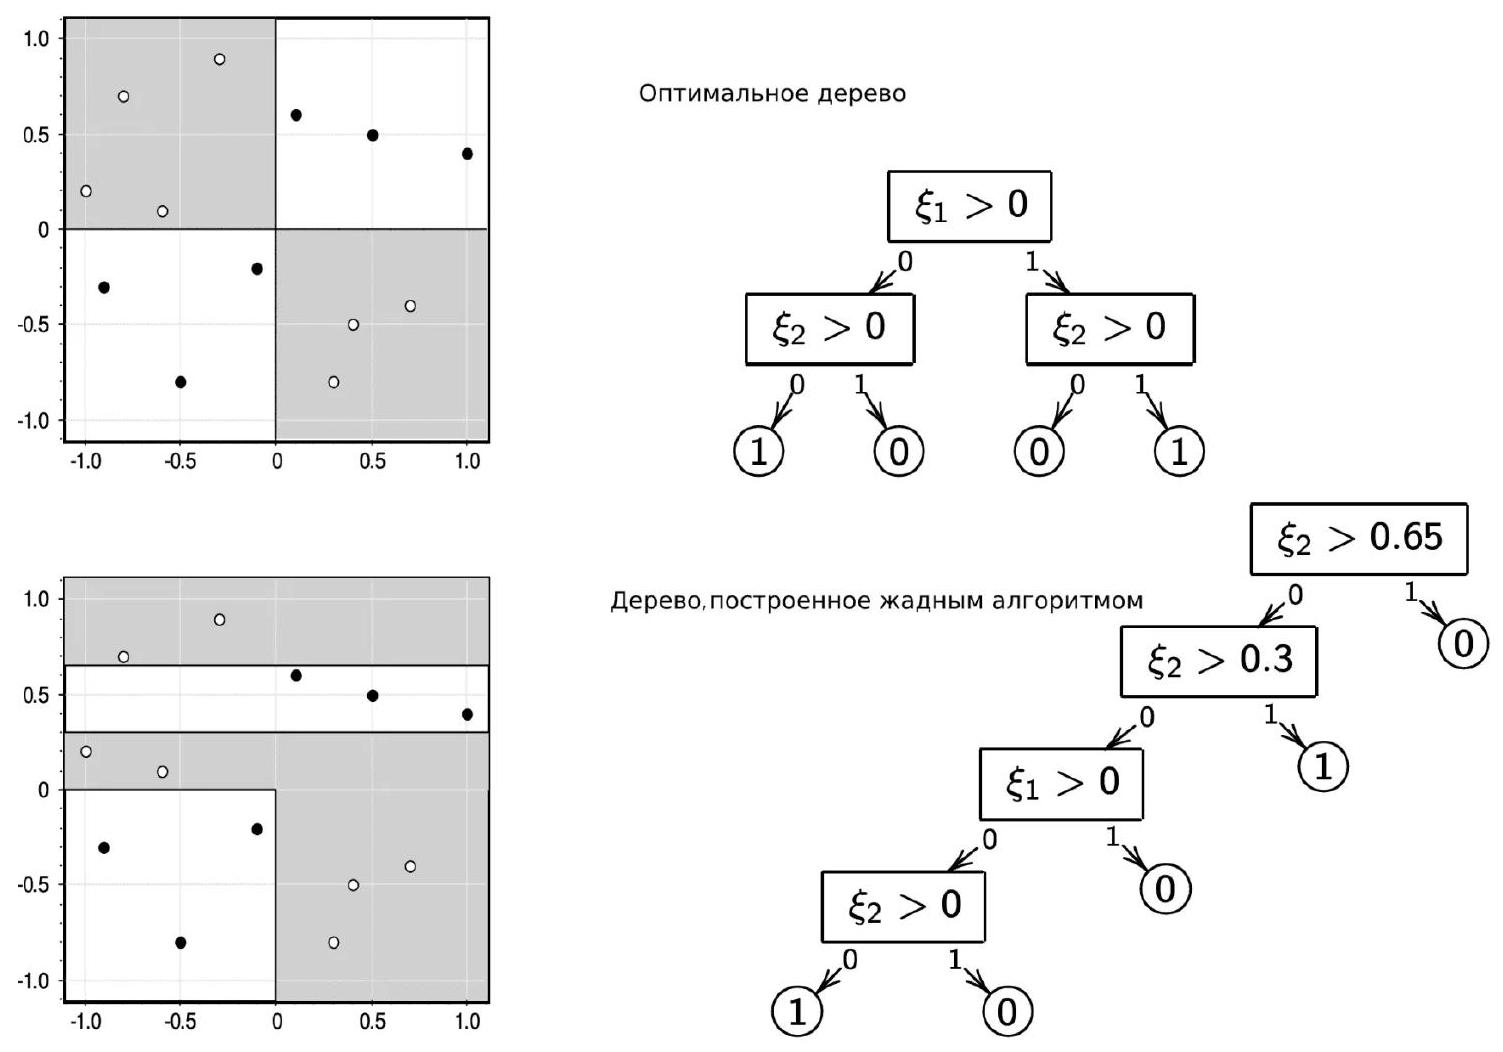
\includegraphics[width=\textwidth, center]{2024_12_13_74602cb5a186ed81f4bcg-8}

Вне зависимости от того, что вы оптимизируете, жадный алгоритм не даст оптимального решения задачи XOR. Но этим примером проблемы не исчерпываются. Скажем, бывают ситуации, когда оптимальное с точки зрения выбранной метрики дерево вы получите с критерием ветвления, построенным по другой метрике (например, MSE-критерий для MAE-задачи или Джини для misclassification error).


\subsection*{Задача 1. Информативность в задаче регрессии (MSE)}

Пусть в лист \(X_m\) попали объекты \(\{(x_i, y_i)\}_{i=1}^n\), и мы рассматриваем критерий информативности для задачи регрессии с квадратичной функцией потерь. Покажите, что минимизация средней квадратичной ошибки в листе приводит к выбору среднего значения таргета \(\overline{y}\) в качестве предсказания, а сама информативность листа равна дисперсии ответов в этом листе. Формально, если

\[
H(X_m) = \frac{1}{n} \sum_{i=1}^n (y_i - c)^2,
\]

то найдите \(c\), минимизирующее \(H(X_m)\), и подставив его обратно, выразите \(H(X_m)\) через \(\overline{y}\) и \(\{y_i\}\).

\subsubsection*{Решение к Задаче 1}

Для функции

\[
H(X_m) = \frac{1}{n} \sum_{i=1}^n (y_i - c)^2
\]

найдём минимум по \(c\). Рассчитаем производную:

\[
\frac{\partial H}{\partial c} = \frac{2}{n} \sum_{i=1}^n (c - y_i).
\]

Приравнивая её к нулю:

\[
\sum_{i=1}^n (c - y_i) = 0 \implies nc - \sum_{i=1}^n y_i = 0 \implies c = \frac{1}{n}\sum_{i=1}^n y_i = \overline{y}.
\]

Таким образом, оптимальное предсказание — среднее значение таргета. Подставляя \(c = \overline{y}\) в \(H(X_m)\), получаем:

\[
H(X_m) = \frac{1}{n} \sum_{i=1}^n (y_i - \overline{y})^2.
\]

Заметим, что это именно выборочная дисперсия (без нормировки на \(n-1\)) таргетов в листе. Таким образом, минимизация MSE соответствует минимизации дисперсии в листьях.


\subsection*{Задача 2. Критерии информативности в задаче классификации}

Пусть в листе \(X_m\) выборки для задачи классификации имеется \(K\) классов, а доля \(k\)-го класса равна \(p_k\). Покажите, что для следующих критериев информативности минимизирующий их вектор вероятностей \(c = (c_1, \ldots, c_K)\) равен \(p = (p_1, \ldots, p_K)\):

1. Ошибка классификации (misclassification error): 
\[
H(X_m) = 1 - \max_k p_k.
\]

2. Энтропия:
\[
H(X_m) = -\sum_{k=1}^K p_k \log p_k.
\]

3. Критерий Джини:
\[
H(X_m) = \sum_{k=1}^K p_k(1 - p_k).
\]

Поясните, почему для всех этих критериев наилучшее предсказание в листе — это вектор оценочных вероятностей классов, равных их эмпирическим частотам.

\subsubsection*{Решение к Задаче 2}

Рассмотрим три критерия информативности.

1. \textbf{Ошибка классификации}: 
Оптимальное предсказание — класс, встречающийся чаще всего, поскольку минимизируется число ошибок. Индикаторная функция ошибки достигает минимума при выборе класса \(k_*\), для которого \(p_{k_*} = \max_k p_k\). Но если мы хотим предсказывать распределение, то его оптимальный вариант — вектор, в котором единица стоит на месте наиболее вероятного класса, что соответствует выборочным частотам (для детерминированного предсказания).

2. \textbf{Энтропия}:
Энтропия минимизируется при вырожденном распределении (когда все массы сосредоточены в одной точке), однако в условиях задачи мы хотим получить оценку, согласованную с данными. В постановке с логарифмом правдоподобия оптимальное распределение классов \((c_1,\ldots,c_K)\) при фиксированных \((y_i)\) достигается при \(c_k = p_k\). Строгий вывод следует из решения задачи оптимизации с ограничением \(\sum_k c_k = 1\). Применение метода Лагранжа приводит к тому, что минимум достигается при совпадении \(c_k\) и \(p_k\).

3. \textbf{Критерий Джини}:
Показатель Джини интерпретируется как ожидаемая ошибка при случайной приписке метки объекта согласно предсказанному распределению. Аналогично энтропии, решение задачи оптимизации даёт \(c_k = p_k\).

Во всех трёх случаях оптимальное распределение в листе совпадает с эмпирическими частотами классов. Это связано с тем, что все рассмотренные критерии имеют минимум в точке эмпирического распределения, отражающего фактические данные.


\subsection*{Задача 3. Жадные алгоритмы и их неоптимальность}

Рассмотрим задачу классификации, где истинное решение требует нетривиальной структуры разделяющей поверхности, например задачу XOR. Покажите, что жадный алгоритм построения дерева, независимо от того, используете ли вы критерий энтропии, Джини или ошибку классификации, не сможет за один или два сплита добиться оптимального разделения. Объясните, почему жадность при выборе сплитов может привести к локально оптимальным, но не глобально оптимальным решениям.

\subsubsection*{Решение к Задаче 3}

Задача XOR устроена так, что данные, принадлежащие разным классам, перемешаны таким образом, что никакой простой линейный или однопараметрический сплит не улучшит ситуацию кардинально, если смотреть на локальный шаг. Жадный алгоритм выбирает признак и порог, максимизирующий улучшение критерия информативности в текущий момент, но не учитывает будущую структуру дерева.

При XOR-классификации каждый простой сплит либо оставляет смешанные классы в листьях, либо не даёт существенного выигрыша по критерию информативности. Чтобы идеально решить XOR, дереву потребуется хотя бы несколько уровней разбиений. Однако жадный выбор первого сплита будет неинформативным с точки зрения глобального решения. Таким образом, критерий информативности, основанный на локальных улучшениях, не гарантирует нахождения глобального оптимума.

Такой пример иллюстрирует фундаментальную проблему: оптимизация критерия информативности по листам не решает NP-полную задачу глобального оптимума структуры дерева. Жадный алгоритм может застревать в локальных оптимумах, не достигая оптимального глобального решения.


\section{Решающее дерево}
Среди множества существующих методов классификации особое место занимают решающие деревья.
Можно выделить несколько преимуществ этих моделей.
\begin{enumerate}
    \item \textbf{Простая реализация}: модель представляет собой структуру, напоминающую дерево с узлами и ветвями.
    \item \textbf{Результаты легко интерпретируемы}: решения принимаются на основе последовательных вопросов о характеристиках объектов.
    \item \textbf{Независимость от структуры данных}: решающее дерево может работать как с числовыми, так и с категориальными признаками без предварительной обработки.

\end{enumerate}
Однако, несмотря на множество преимуществ, решающие деревья имеют и некоторые ограничения. Например, они склонны к переобучению, особенно при наличии большого количества признаков или при недостаточной глубине дерева.
Для преодоления этих недостатков были разработаны различные методы регуляризации и оптимизации, позволяющие улучшить общую производительность модели. А так же решающее деревья послужили базой для построения более сложных алгоритмов, таких как градиентный бустинг на деревьях и случайный лес.

\subsection{Моделирование решающих деревьев}
Условимся обозначать через $\mathbb{X}$ множество объектов, поступающих на вход модели, через $\mathbb{Y}$ множество объектов, в которое модель действует. Начнём с определения.
\begin{definition}
    \textit{Решающим деревом} называется бинарное дерево, в котором
    \begin{enumerate}
        \item каждой внутренней вершине $v$ преписан предикат $B_v: \mathbb{X} \to \{0, 1\}$;
        \item каждой листовой вершине $u$ преписан прогноз $c_u \in \mathbb{Y}$.
    \end{enumerate}
\end{definition}

Давайте немного обсудим определение. Во-первых, понятно как получить для входного объекта ответ: применить к нему предикат и, если он равен 1 (0), пойти в правого (левого) сына текущей вершины, а затем повторять процедуру, пока не дошли до листа. Во-вторых, прогнозы, приписанные листовым вершинам, могут иметь любую природу: будь это числовые константы, векторы вероятностей или даже другие модели. Но всё же обычно, останавливаются на предсказании констант (для классификации - номер класса или всё так же вектор вероятностей принадлежности классам).

\begin{example}
    В задаче классификации клиентов банка на категории "кредитоспособный" и "некредитоспособный" решающее дерево может сначала разделить клиентов по уровню дохода, затем по наличию задолженностей и т.д., чтобы в конечном итоге определить вероятность одобрения кредита для каждого клиента.
\end{example}

\subsection{Обучение решающих деревьев}
Процесс обучения решающего дерева включает в себя последовательное разделение данных на подмножества, основываясь на значениях различных признаков, с целью максимизации чистоты классов в каждом узле дерева. А именно, хочется подбирать предикат для каждого узла так, чтобы разбиние данных, доходящих до него, было наилучшим из возможных. Одним из наиболее распространённых подходов к построению решающих деревьев является использование \textit{жадного алгоритма}. Для простоты условимся работать только с так называемыми \textit{пороговыми предикатами}: $B_{j, t} = x_j \leq t$.

Пусть $X$ — обучающая выборка, а $X_m$ — множество объектов в текущем узле (в начале $X_m = X$). Жадный алгоритм строится следующим образом:

\begin{enumerate}
    \item Создаём вершину $v$.
    \item Если выполнен критерий остановки $Stop(X_m)$, объявляем вершину листом с ответом $Ans(X_m)$.
    \item Иначе выбираем предикат $B_{j,t}$, который максимально улучшает критерий ветвления $Branch(X_m, j, t)$, и делим $X_m$ на $X_{\ell}$ и $X_r$.
    \item Для $X_{\ell}$ и $X_r$ повторяем процесс рекурсивно.
\end{enumerate}

Алгоритм использует вспомогательные функции:
\begin{itemize}
    \item $Ans(X_m)$ — ответ в листе. Например, для классификации это самый частый класс или распределение вероятностей, для регрессии — среднее значение, медиана или простая модель.
    \item $Stop(X_m)$ — правило остановки, срабатывающее, если данные в узле достаточно однородны или их слишком мало.
    \item $Branch(X_m, \textit{feature}, \textit{value})$ — оценка качества разбиения. Выбирается предикат, дающий наибольшее улучшение.
\end{itemize}

Как правило, $Ans(X_m)$ и $Branch(X_m, \textit{feature}, \textit{value})$ подбираются во время обучения дерева, а функция $Stop(X_m)$ выступает гиперпараметром построения этого дерева.
Самым интересным является подборр функции для узла, обеспечивающий наилучшее разбиение. Об этом стоит поговорить подробнее.

\subsection{Критерии ветвления}
Ответы дерева можно представлять в виде $c \in \mathbb{R}$ для задач регрессии и меток классов. В случаях, когда требуется предсказать вероятностное распределение классов, $c$ будет вектором вероятностей, то есть $c \in \mathbb{R}^K$:

\[
c = (c_1, \dots, c_K), \quad \sum_{i=1}^K c_i = 1
\]

Предположим, что задана функция потерь $L(y_i, c)$, которая измеряет качество предсказаний.

При поиске оптимального разбиения $X_m = X_\ell \bigsqcup X_r$ можно вычислить константное значение $c$, которое предсказало бы дерево, если текущая вершина стала бы листом. Это значение выбирается так, чтобы минимизировать среднее значение функции потерь:

\[
\frac{1}{|X_m|} \sum_{(x_i, y_i) \in X_m} L(y_i, c)
\]

Минимальное значение этой функции:

\[
H(X_m) = \min_{c \in Y} \frac{1}{|X_m|} \sum_{(x_i, y_i) \in X_m} L(y_i, c)
\]

называют информативностью или \textit{impurity}. Чем ниже эта величина, тем лучше объекты внутри листа аппроксимируются константным значением.

Критерий ветвления определяется через изменение информативности следующим образом:

\[
Branch(X_m, j, t) = |X_m| \cdot H(X_m) - |X_\ell| \cdot H(X_\ell) - |X_r| \cdot H(X_r)
\]

Интуция здесь следующая: мы смотрим, как хорошо можно приблизить объекты константным значением, если разбить их на две части (естественно константы свои для каждой части), и сравниваем это с информативностью, которую имеем на данный момент.

Получившаяся величина неотрицательна: ведь, разделив объекты на две кучки и подобрав ответ для каждой, мы точно не сделаем хуже. Кроме того, она тем больше, чем лучше предлагаемый сплит.

Остаётся определить функционал качества $L$ и можно обучать дерево. Но для задачи классификации можно определить информативность немного по-другому, что снова заслуживает небольшого отдельного разговора.

\subsection{Энтропия}
Если необходимо предсказывать вероятностное распределение классов $(c_1, \dots, c_K)$, это можно сделать аналогично логистической регрессии. Основной подход заключается в максимизации логарифма правдоподобия (или минимизации его отрицательной величины) для распределения Бернулли. Предположим, что в вершине дерева предсказывается фиксированное распределение $c$, которое не зависит от $x_i$. В этом случае правдоподобие выражается следующим образом:

\[
P(y \mid x, c) = P(y \mid c) = \prod_{(x_i, y_i) \in X_m} P(y_i \mid c) = \prod_{(x_i, y_i) \in X_m} \prod_{k=1}^K c_k^{\mathbb{I}[y_i = k]},
\]

откуда вытекает, что
,
\[
H(X_m) = \min_{\sum_k c_k = 1} \left( -\frac{1}{|X_m|} \sum_{(x_i, y_i) \in X_m} \sum_{k=1}^K \mathbb{I}[y_i = k] \log c_k \right).
\]

\section{Задачи для закрепления материала}
\subsection{Задача 1: Переобучение дерева}
Пусть у вас есть тренировочная выборка из 100 объектов с 10 признаками и тестовая выборка из 30 объектов. Вы построили решающее дерево, которое идеально классифицирует тренировочную выборку (точность 100\%), но на тестовой выборке точность всего 50\%.

\textbf{Вопросы}:
\begin{enumerate}
    \item Почему произошло переобучение?
    \item Какие методы регуляризации можно применить, чтобы уменьшить переобучение?
    \item Как критерий остановки помогает предотвратить переобучение?
\end{enumerate}
\begin{solution}
Причина: дерево слишком сложное (глубокое), оно идеально подстроилось под тренировочные данные, но на тестовых данные из-за слабой обобщающей способности модель показала низкий результат.

Варинты решений:
\begin{enumerate}
    \item Ограничить максимальную глубину (\(\texttt{max\_depth}\)).
    \item Установить минимальное число объектов в листе (\(\texttt{min\_samples\_leaf}\)).
    \item Использовать случайный лес или ансамбли для повышения обобщающей способности.
\end{enumerate}
\end{solution}

\subsection{Задача 2: Вывод энтропийного критерия}
Вернёмся к последнему пункту, а конкретнее к информативности, предложенной в нём:
\[
H(X_m) = \min_{\sum_k c_k = 1} \left( -\frac{1}{|X_m|} \sum_{(x_i, y_i) \in X_m} \sum_{k=1}^K \mathbb{I}[y_i = k] \log c_k \right).
\]
Но причём же тут энтропия? Докажите, что что оценка вероятностей в листе $c_{k}$, минимизирующая $H(X_M)$, должна быть равна $p_k$, то есть доле попавших в лист объектов этого класса. Откуда при подстановке вектора вероятностей $c = (c_1, \dots, c_K)$ получается формула
\[
H(X_m) = - \sum_{k=1}^K p_k \log p_k
\]
\begin{solution}
    Из-за наличия условия $\sum_k c_k = 1$ нам придётся минимизировать лагранжиан:

\[
L(c, \lambda) = \min_{c, \lambda} \left( -\frac{1}{|X_m|} \sum_{(x_i, y_i) \in X_m} \sum_{k=1}^K \mathbb{I}[y_i = k] \log c_k + \lambda \sum_{k=1}^K c_k \right).
\]

Как обычно, возьмём частную производную по $c_j$ и решим уравнение:

\[
0 = \frac{\partial}{\partial c_j} L(c, \lambda) =
\]

\[
= \frac{\partial}{\partial c_j} \left( -\frac{1}{|X_m|} \sum_{(x_i, y_i) \in X_m} \sum_{k=1}^K \mathbb{I}[y_i = k] \log c_k + \lambda \sum_{k=1}^K c_k \right).
\]

Упрощаем производную:

\[
0 = \left( -\frac{1}{|X_m|} \sum_{(x_i, y_i) \in X_m} \mathbb{I}[y_i = j] \frac{1}{c_j} \right) + \lambda.
\]

Решая уравнение относительно $c_j$, получаем:

\[
c_j = \frac{p_j}{\lambda},
\]

где $p_j = \frac{1}{|X_m|} \sum_{(x_i, y_i) \in X_m} \mathbb{I}[y_i = j]$ — доля объектов класса $j$ в текущем узле.

Суммируя эти равенства по $j$, учитывая, что $\sum_k c_k = 1$, находим значение $\lambda$:

\[
1 = \sum_{k=1}^K c_k = \frac{1}{\lambda} \sum_{k=1}^K p_k = \frac{1}{\lambda}.
\]

Таким образом, $\lambda = 1$, и окончательное выражение для $c_j$ имеет вид:

\[
c_j = p_j,
\]

то есть оптимальное значение $c_j$ — это доля объектов класса $j$ в узле $X_m$.
\end{solution}

\subsection{Задача 3: Построение простого дерева}
Дан набор данных:

\[
\begin{array}{|c|c|c|c|}
\hline
\textbf{Объект} & \textbf{Признак 1} & \textbf{Признак 2} & \textbf{Класс} \\
\hline
1 & 5 & 10 & A \\
2 & 6 & 15 & A \\
3 & 7 & 20 & B \\
4 & 8 & 25 & B \\
\hline
\end{array}
\]

Попробуйте построить вручную решающее дерево для классификации этих объектов. Используйте пороговые предикаты вида $B_{j, t} = x_j \leq t$. А в качестве критерия информативности используйте \textit{индекс Джини}

\[
Gini(X_m) = 1 - \sum_{k=1}^K p_k^2,
\]

где $p_k$ — доля объектов класса $k$ в $X_m$.

\textbf{Вопросы}:
\begin{itemize}
    \item Какие пороговые значения для признаков вы выбрали?
    \item Какой индекс Джини у корневого узла и у каждого листа?
\end{itemize}

\begin{solution}
\subsubsection*{Шаг 1: Рассчитаем индекс Джини для всего набора данных}
    В исходной выборке два класса: $A$ и $B$, каждый представлен двумя объектами. Тогда:

\[
p_A = \frac{2}{4} = 0.5, \quad p_B = \frac{2}{4} = 0.5.
\]

Индекс Джини для всего набора:

\[
Gini(X) = 1 - p_A^2 - p_B^2 = 1 - 0.5^2 - 0.5^2 = 1 - 0.25 - 0.25 = 0.5.
\]

\subsubsection*{Шаг 2: Разделение по признаку 1 с порогом $x_1 \leq 6$}

Разделение выборки:
\begin{itemize}
    \item Левая часть $X_\ell$: объекты 1, 2 (\textbf{Класс A}).
    \item Правая часть $X_r$: объекты 3, 4 (\textbf{Класс B}).
\end{itemize}

\noindent Рассчитаем индексы Джини для каждой части:
\begin{itemize}
    \item Для $X_\ell$:
    \[
    p_A = 1, \quad p_B = 0, \quad Gini(X_\ell) = 1 - 1^2 - 0^2 = 0.
    \]

    \item Для $X_r$:
    \[
    p_B = 1, \quad p_A = 0, \quad Gini(X_r) = 1 - 1^2 - 0^2 = 0.
    \]
\end{itemize}

\subsubsection*{Шаг 3: Совокупный индекс Джини для разбиения}

Совокупный индекс Джини рассчитывается как:

\[
Gini_{split} = \frac{|X_\ell|}{|X|} Gini(X_\ell) + \frac{|X_r|}{|X|} Gini(X_r),
\]

где $|X_\ell|$ и $|X_r|$ — размеры левой и правой частей соответственно. Подставим значения:

\[
Gini_{split} = \frac{2}{4} \cdot 0 + \frac{2}{4} \cdot 0 = 0.
\]

\subsubsection*{Шаг 4: Итоговое дерево}

Порог $x_1 \leq 6$ полностью разделяет данные на два класса $A$ и $B$, минимизируя индекс Джини. Дерево имеет следующую структуру:

\begin{itemize}
    \item Если $x_1 \leq 6$, то $Класс = A$.
    \item Если $x_1 > 6$, то $Класс = B$.
\end{itemize}

\subsubsection*{Ответы на вопросы:}

\begin{itemize}
    \item Выбранный порог для признака 1: $x_1 \leq 6$.
    \item Индекс Джини у корневого узла: $0.5$.
    \item Индекс Джини у листов: $0$.
\end{itemize}
\end{solution}

\section*{Точный тест Фишера}

\textbf{Точный тест Фишера} — это тест статистической значимости, используемый в анализе категориальных данных, когда размеры выборки малы (являются маленькими). Назван в честь его изобретателя, Р. А. Фишера, и является одним из класса точных тестов. Фишер разрабатывал тест после комментария от Muriel Bristol, которая утверждала, будто была в состоянии обнаружить, были ли чай или молоко добавлены сначала в её чашку.

Тест обычно используется, чтобы исследовать значимость взаимосвязи между двумя переменными в факторной таблице размерности $2 \times 2$ (таблице сопряжённости признаков). Величина вероятности $P$ теста вычисляется, как если бы значения на границах таблицы известны. Например, в случае с дегустацией чая, госпожа Bristol знает число чашек с каждым способом приготовления (молоко или чай сначала), поэтому якобы предоставляет правильное число угадываний в каждой категории. Как было указано Фишером, в предположении нуль-гипотезы о независимости испытаний это ведёт к использованию гипергеометрического распределения для данного счёта в таблице.

С большими выборками в этой ситуации может использоваться тест хи-квадрат. Однако этот тест не является подходящим, когда математические ожидания значений в любой из ячеек таблицы с заданными границами оказываются ниже 10: вычисленное выборочное распределение испытуемой статистической величины только приблизительно равно теоретическому распределению хи-квадрат, и приближение неадекватно в этих условиях (которые возникают, когда размеры выборки малы или данные очень неравноценно распределены среди ячеек таблицы). Тест Фишера, как следует из его названия, является точным и может, поэтому, использоваться независимо от особенностей выборки. Тест становится трудно вычислимым для больших выборок или хорошо уравновешенных таблиц, но, к счастью, именно для этих условий хорошо применим критерий хи-квадрат.

Для ручных вычислений тест выполним только в случае размерности факторных таблиц $2 \times 2$. Однако принцип теста может быть расширен на общий случай таблиц $m \times n$, и некоторые статистические пакеты обеспечивают такие вычисления (иногда используя метод Монте-Карло, чтобы получить приближение).

\section*{Пример}

Точные тесты позволяют получать более аккуратный анализ для маленьких выборок или данных, которые редки. Точные тесты непараметрических исследований являются подходящим статистическим инструментом для работы с неуравновешенными данными. Неуравновешенные данные, проанализированные асимптотическими методами, имеют тенденцию приводить к ненадёжным результатам. Для больших и хорошо уравновешенных наборов данных точные и асимптотические оценки вероятностей $P$ очень похожи. Но для маленьких, редких или выведенных из равновесия данных точные и асимптотические оценки могут быть весьма различными и даже привести к противоположным заключениям относительно разрабатываемой гипотезы.

Потребность в тесте Фишера возникает, когда у нас есть данные, разделённые на две категории двумя отдельными способами. Например, выборка подростков может быть разделена на категории с одной стороны по признаку пола (юноши и девушки), а с другой стороны — по признаку нахождения на диете или нет. Можно выдвинуть гипотезу, что доля находящихся на диете людей выше среди девушек, чем среди юношей, и мы хотим удостовериться, является ли какое-нибудь наблюдаемое различие пропорций статистически значимым.

Данные могли бы быть такими:

\begin{center}
\begin{tabular}{|c|c|c|c|}
\hline
              & Юноши & Девушки & Всего \\
\hline
На диете      & 1     & 9       & 10 \\
\hline
Не на диете   & 11    & 3       & 14 \\
\hline
Всего         & 12    & 12      & 24 \\
\hline
\end{tabular}
\end{center}

Такие данные не подходят для анализа методом хи-квадрат, потому что математические ожидания в таблице — все ниже 10. 

Фишер показал, что вероятность получения любого такого набора величин даётся гипергеометрическим распределением:

\[
P = \frac{\binom{a+b}{a} \binom{c+d}{c}}{\binom{n}{a+c}} = \frac{(a+b)!(c+d)!(a+c)!(b+d)!}{n!a!b!c!d!},
\]

где $\binom{n}{k}$ — биномиальные коэффициенты, а $!$ указывает оператор факториала.

Эта формула даёт точную вероятность наблюдения любого специфического набора данных при условии заданных маргинальных итогов, общего итога и нулевой гипотезы об одинаковой предрасположенности к диете независимо от пола.

Для оценки статистической значимости наблюдаемых данных вычисляют значение $P$ для всех таблиц с такими же маргинальными итогами, что и в исходной таблице, и суммируют вероятности для случаев с такими же или более выраженными различиями.

\section*{Примеры задач}

\subsection*{Задача 1: Оценка влияния лекарственного препарата}

Исходные данные:
\[
\begin{array}{|c|c|c|c|}
\hline
                 & \text{Улучшение} & \text{Нет улучшения} & \text{Всего} \\
\hline
\text{Препарат}  & 8                & 2                    & 10 \\
\hline
\text{Плацебо}   & 3                & 7                    & 10 \\
\hline
\text{Всего}     & 11               & 9                    & 20 \\
\hline
\end{array}
\]

Рассчитываем вероятность $P$:
\[
P = \frac{\binom{10}{8} \binom{10}{3}}{\binom{20}{11}}
\]
Рассчитаем биномиальные коэффициенты:
\[
\binom{10}{8} = 45, \quad \binom{10}{3} = 120, \quad \binom{20}{11} = 167960.
\]
Подставляем значения:
\[
P = \frac{45 \cdot 120}{167960} \approx 0.0321.
\]
\textbf{Результат}: Значение $P \approx 0.0321$ меньше уровня значимости $\alpha = 0.05$, поэтому нулевая гипотеза (о том, что препарат не влияет на улучшение состояния) отклоняется. Препарат оказывает статистически значимое влияние.

\subsection*{Задача 2: Пол и выбор профессии}

Исходные данные:
\[
\begin{array}{|c|c|c|c|}
\hline
                 & \text{Инженеры} & \text{Гуманитарии} & \text{Всего} \\
\hline
\text{Мужчины}   & 15              & 5                  & 20 \\
\hline
\text{Женщины}   & 4               & 16                 & 20 \\
\hline
\text{Всего}     & 19              & 21                 & 40 \\
\hline
\end{array}
\]

Рассчитываем вероятность $P$:
\[
P = \frac{\binom{20}{15} \binom{20}{4}}{\binom{40}{19}}
\]
Рассчитаем биномиальные коэффициенты:
\[
\binom{20}{15} = 15504, \quad \binom{20}{4} = 4845, \quad \binom{40}{19} = 68923264410.
\]
Подставляем значения:
\[
P = \frac{15504 \cdot 4845}{68923264410} \approx 0.0011.
\]
\textbf{Результат}: Значение $P \approx 0.0011$ значительно меньше уровня значимости $\alpha = 0.05$, поэтому нулевая гипотеза (о независимости пола и выбора профессии) отклоняется. Пол имеет значимое влияние на выбор профессии.

\subsection*{Задача 3: Эксперимент с дегустацией чая}

Исходные данные:
\[
\begin{array}{|c|c|c|c|}
\hline
                 & \text{Чай первым} & \text{Молоко первым} & \text{Всего} \\
\hline
\text{Угадано верно}    & 3                  & 2                    & 5 \\
\hline
\text{Угадано неверно}  & 1                  & 2                    & 3 \\
\hline
\text{Всего}            & 4                  & 4                    & 8 \\
\hline
\end{array}
\]

Рассчитываем вероятность $P$:
\[
P = \frac{\binom{5}{3} \binom{3}{1}}{\binom{8}{4}}
\]
Рассчитаем биномиальные коэффициенты:
\[
\binom{5}{3} = 10, \quad \binom{3}{1} = 3, \quad \binom{8}{4} = 70.
\]
Подставляем значения:
\[
P = \frac{10 \cdot 3}{70} = 0.4286.
\]
\textbf{Результат}: Значение $P \approx 0.4286$ значительно больше уровня значимости $\alpha = 0.05$, поэтому нулевая гипотеза (о случайности угадывания) не отвергается. Испытуемый, вероятно, угадывает случайным образом.

\section{Oblique Random Forest and Rotation Forest}
В последние годы методы ансамблевого обучения, такие как Random Forest, получили широкое распространение благодаря своей высокой эффективности и устойчивости к переобучению. Однако, существуют различные модификации этих методов, которые могут улучшить их производительность. В данной работе рассматриваются два таких метода: Oblique Random Forest и Rotation Forest.

\section{Oblique Random Forest}
Oblique Random Forest (ORF) представляет собой модификацию классического Random Forest, в которой используются обlique (косые) разбиения для создания деревьев решений. В отличие от традиционных деревьев, которые принимают решения на основе вертикальных разбиений (параллельных осям), ORF использует линейные комбинации признаков для разделения данных.

\subsection{Преимущества}
\begin{itemize}
    \item Более гибкие разбиения, позволяющие лучше захватывать сложные зависимости в данных.
    \item Увеличение точности модели за счет использования линейных комбинаций признаков.
\end{itemize}

\subsection{Примеры применения}
Обlique Random Forest может быть полезен в задачах, где данные имеют сложные структуры, такие как:
\begin{itemize}
    \item Классификация изображений.
    \item Анализ текстовых данных.
    \item Финансовый анализ, где зависимости между признаками могут быть нелинейными.
\end{itemize}

\section{Rotation Forest}
Rotation Forest (RoF) является еще одной модификацией Random Forest, которая использует метод вращения признаков для улучшения производительности модели. В этом методе каждый базовый классификатор обучается на подмножестве данных, которое предварительно преобразуется с помощью метода главных компонент (PCA) или других методов вращения.

\subsection{Преимущества}
\begin{itemize}
    \item Устойчивость к переобучению за счет уменьшения корреляции между деревьями.
    \item Возможность выявления скрытых структур в данных благодаря преобразованию признаков.
\end{itemize}

\subsection{Примеры применения}
Rotation Forest может быть использован в различных областях, таких как:
\begin{itemize}
    \item Биомедицинская диагностика, где важно учитывать взаимодействия между множеством признаков.
    \item Финансовые прогнозы, где необходимо учитывать множество факторов.
    \item Обработка естественного языка, где важно учитывать контекст и семантику.
\end{itemize}

\title{Задачи по Oblique Random Forest и Rotation Forest}
\author{}
\date{}
\maketitle

\subsection*{Задача 1: Обнаружение мошенничества с использованием Oblique Random Forest}

\textbf{Условие:} 
Вам даны данные о транзакциях, содержащие различные признаки, такие как сумма транзакции, местоположение и т.д. Необходимо определить, является ли транзакция мошеннической. Данные имеют высокую размерность и много коррелирующих признаков.

\textbf{Решение:}
Используем метод Oblique Random Forest, который позволяет строить наклонные деревья решений. Это может помочь лучше захватить сложные зависимости между признаками.

1. Подготовка данных: нормализация и кодирование категориальных переменных.
2. Разделение данных на обучающую и тестовую выборки.
3. Обучение Oblique Random Forest на обучающей выборке.
4. Оценка качества модели с использованием метрик, таких как F1-score и ROC-AUC.

\textbf{Формула для оценки качества:}
\[
F1 = 2 \cdot \frac{\text{Precision} \cdot \text{Recall}}{\text{Precision} + \text{Recall}}
\]

\section{Задачи}

\subsection*{Задача 2: Классификация изображений с использованием Rotation Forest}

\textbf{Условие:} 
Имеется набор изображений, которые необходимо классифицировать по категориям (например, животные, растения и т.д.). Изображения имеют высокую размерность и могут содержать много шумов.

\textbf{Решение:}
Используем метод Rotation Forest, который создает несколько подвыборок и применяет метод главных компонент (PCA) для уменьшения размерности и поворота признаков.

1. Разделение данных на обучающую и тестовую выборки.
2. Для каждой подвыборки:
   - Применение PCA для уменьшения размерности.
   - Обучение базового классификатора (например, Decision Tree).
3. Объединение результатов классификации всех базовых классификаторов.

\textbf{Формула для PCA:}
\[
Z = XW
\]
где \(Z\) - матрица преобразованных данных, \(X\) - исходная матрица данных, \(W\) - матрица весов (векторы главных компонент).

\subsection*{Задача 3: Прогнозирование временных рядов с использованием Oblique Random Forest}

\textbf{Условие:} 
Необходимо предсказать значения временного ряда (например, продажи товаров) на основе исторических данных. Данные имеют временные зависимости и могут быть нестационарными.

\textbf{Решение:}
Применяем Oblique Random Forest, чтобы учитывать сложные зависимости между временными признаками.

1. Подготовка данных: создание временных признаков (например, лаги, скользящие средние).
2. Разделение данных на обучающую и тестовую выборки.
3. Обучение Oblique Random Forest на обучающей выборке.
4. Прогнозирование на тестовой выборке и оценка качества с помощью RMSE.

\textbf{Формула для RMSE:}
\[
RMSE = \sqrt{\frac{1}{n} \sum_{i=1}^{n} (y_i - \hat{y}_i)^2}
\]
где \(y_i\) - истинные значения, \(\hat{y}_i\) - предсказанные значения.

\section{Заключение}
Oblique Random Forest и Rotation Forest представляют собой мощные инструменты для решения задач классификации и регрессии. Их применение может значительно повысить точность моделей, особенно в сложных и многомерных данных.

\end{document}
